%%% Template File for Use with the hmcclinic.cls.
%%%
%%% C.M. Connelly <cmc@math.hmc.edu>
%%%  $Id: clinic-template.tex 368 2011-08-01 18:53:50Z cmc $
%%%
%%%  Tag: $Name$


%%% !!! HMC STUDENTS SHOULD REMOVE THE FOLLOWING COPYRIGHT NOTICE FROM
%%% !!! FINAL SUBMISSIONS.

%%% Copyright (C) 2004-2010 Department of Mathematics, Harvey Mudd College.

%%% See the COPYING document, which should accompany this
%%% distribution, for information about distribution and modification
%%% of the document and its components.

%%% !!! END COPYRIGHT NOTICE.

%%%%%%%%%%%%%%%%%%%%%%%%%%%%%%%%%%%%%%%%%%%%%%%%%%%%%%%%%%%%%%%%%%%%%%
%%% Note that for your Clinic report, you should remove any        %%%
%%% comments that aren't relevant to your report.  You should also %%%
%%% remove the copyright notice assigning copyright to the         %%%
%%% department (depending on your sponsor, you may need to assign  %%%
%%% copyright to the sponsoring organization).                     %%%
%%%%%%%%%%%%%%%%%%%%%%%%%%%%%%%%%%%%%%%%%%%%%%%%%%%%%%%%%%%%%%%%%%%%%%

%%% Preamble.

%%% The top part of your document is called the preamble.  You supply
%%% some basic information about the document (such as its title and
%%% author) in a form that LaTeX can understand here.


%%% The first active line in your LaTeX document is the \documentclass
%%% command, which loads a LaTeX class file.  Class files generally
%%% define the appearance of a document, and include a variety of
%%% structural commands.

%%% Clinic reports use the clinic class, which should be located
%%% somewhere in TeX's search path.

%%% For midyear reports, include the midyear option, as in
%%%   \documentclass[midyear]{hmcclinic}
\documentclass{hmcclinic}

%%% You can also load additional LaTeX packages, or style files, that
%%% affect the way that the document is laid out, typeset, or supply
%%% additional commands or environments.  If you choose to load
%%% additional packages, make sure that they appear *before* the
%%% line loading hyperref; hyperref changes pieces of other
%%% packages, so it's important that it be loaded last.

\usepackage{graphicx}           % More control over graphic inclusion.
% \usepackage{amsthm}             % AMS theorem styles
\setcounter{tocdepth}{2}
\usepackage{comment}
\usepackage{listings}
\usepackage[section]{placeins}
\usepackage{float}
\sloppypar

\makeatletter
\AtBeginDocument{%
  \expandafter\renewcommand\expandafter\subsection\expandafter{%
    \expandafter\@fb@secFB\subsection
  }%
}
\makeatother

\usepackage{caption}
\lstset{language=C++}


% listings settings from http://en.wikibooks.org/wiki/LaTeX/Source_Code_Listings
\usepackage{color}

\definecolor{mygreen}{rgb}{0,0.6,0}
\definecolor{mygray}{rgb}{0.5,0.5,0.5}
\definecolor{mymauve}{rgb}{0.58,0,0.82}
\lstset{ %
  backgroundcolor=\color{white},   % choose the background color; you must add \usepackage{color} or \usepackage{xcolor}
  basicstyle=\footnotesize,        % the size of the fonts that are used for the code
  breakatwhitespace=false,         % sets if automatic breaks should only happen at whitespace
  breaklines=true,                 % sets automatic line breaking
  captionpos=b,                    % sets the caption-position to bottom
  commentstyle=\color{mygreen},    % comment style
  deletekeywords={...},            % if you want to delete keywords from the given language
  escapeinside={\%*}{*)},          % if you want to add LaTeX within your code
  extendedchars=true,              % lets you use non-ASCII characters; for 8-bits encodings only, does not work with UTF-8
  frame=single,                    % adds a frame around the code
  keepspaces=true,                 % keeps spaces in text, useful for keeping indentation of code (possibly needs columns=flexible)
  keywordstyle=\color{blue},       % keyword style
  language=C++,                 % the language of the code
  otherkeywords={*,...},            % if you want to add more keywords to the set
  numbers=left,                    % where to put the line-numbers; possible values are (none, left, right)
  numbersep=5pt,                   % how far the line-numbers are from the code
  numberstyle=\tiny\color{mygray}, % the style that is used for the line-numbers
  rulecolor=\color{black},         % if not set, the frame-color may be changed on line-breaks within not-black text (e.g. comments (green here))
  showspaces=false,                % show spaces everywhere adding particular underscores; it overrides 'showstringspaces'
  showstringspaces=false,          % underline spaces within strings only
  showtabs=false,                  % show tabs within strings adding particular underscores
  stepnumber=1,                    % the step between two line-numbers. If it's 1, each line will be numbered
  stringstyle=\color{mymauve},     % string literal style
  tabsize=2,                       % sets default tabsize to 2 spaces
  title=\lstname                   % show the filename of files included with \lstinputlisting; also try caption instead of title
}






%%% Load all other packages before this point.

%%% Load hyperref.
\usepackage[breaklinks=true,
  bookmarks,
  pdfpagemode=UseOutlines,
  pdfpagelayout=SinglePage]{hyperref}


%%% The preamble can also be used to define your own commands and
%%% environments, set some constants that will be used throughout your
%%% document, and so on.

%%% As you may have guessed, LaTeX's comment character is the percent
%%% sign.  Any line that starts with a % will be ignored.  You can
%%% also use the comment character to add comments to the end of a
%%% line that will be parsed by TeX.

%%% The optional \includeonly command allows you to specify the names
%%% of chapters that you want to typeset.  It is useful for debugging
%%% or for working intensely on one particular part of your document
%%% when you don't want to take the time to retypeset the entire document.


%%% This optional command provides additional context around an error.
%%% It can be helpful when tracking down a problem. 
%\setcounter{errorcontextlines}{1000}


%%% Information about this document.

%%% I find it most useful to put identifying information about a
%%% document near the top of the preamble.  Technically, this
%%% information must precede the \maketitle command, which often
%%% appears immediately after the beginning of the document 
%%% environment.  Placing it near the top of the document makes it
%%% easier to identify the document, and keeps it from getting
%%% mixed up with the content of your document.

%%% So, some questions.

%% What is the name of the company or organization sponsoring your project?
\sponsor{Sandia National Laboratories}

%% What is the title of your report?
\title{Parallelizing Intrepid Tensor Contractions Using Kokkos}

%% Who are the authors of the report (your team members)?  (Separate
%% names with \and.)
\author{Brett Collins~(Project Manager) \and Alex Gruver \and Ellen Hui \and
Tyler Marklyn}

%% What is your faculty advisor's name?  (Again, separate names with
%% \and, if necessary.)
\advisor{Jeff Amelang}

%% Liaison's name or names?
\liaison{H. Carter Edwards and Robert J. Hoekstra}

%% By not specifying a date with the \date command, the date the
%% document is typeset will be added.

%% If you need to put in a specific date, do so with
%%  \date{May 13, 2004}
%% You probably shouldn't, however.

%%% End of information section.


%%% New commands and environments.

%%% You can define your own commands and environments here.  If you
%%% have a lot of material here, you might want to consider splitting
%%% the commands and environments into a separate ``style'' file that
%%% you load with \usepackage.

% \newcommand{\coolcommand}[1]{#1 is cool.} % Lets everyone know that
                                % the person or thing that you provide
                                % as the argument to the command is
                                % cool.

% \newcounter{cms}


%%% Some theorem-like command definitions.

%%% The \newtheorem command comes from the amsthm package.  That
%%% package is *not* loaded by the class file, so if you choose
%%% to use these commands, you'll need to load the package above.

% \newtheorem{thm}{Theorem}[chapter]
% \newtheorem{lem}{Lemma}[chapter]


%%% If you find that some words in your document are being hyphenated
%%% incorrectly, you can specify the correct hyphenation using the
%%% \hyphenation command.  Note that words are separated by
%%% whitespace, as shown below.

\hyphenation{ap-pen-dix wer-ther-i-an}


%%% The start of the document!

%% The document environment is the main environment in any LaTeX
%% document.  It contains other environments, as well as your text.

\begin{document}

%%% The front matter of a large document includes the title page or
%%% pages, tables of contents, lists of figures or tables, and so on,
%%% your abstract, a preface or introduction, and so on.  It's
%%% delineated with the \frontmatter command.

\frontmatter


%%% One of the things that the \frontmatter does is make page
%%% numbers appear as lowercase Roman numerals---i, vi, xii, and so
%%% on.

%%% The first thing in the front matter is your title page.  The title
%%% page is formatted by commands in the document class file, so you
%%% don't need to worry about what it looks like -- just putting the
%%% \maketitle command in your document (and filling in the necessary
%%% information for the identification commands above) is enough.

\maketitle


%%% Abstract

\begin{abstract}
  As computer hardware capabilities increase, code parallelism is becoming
  an increasingly vital part of writing high-performing, computationally
  expensive code such as that used in scientific computing.  Some problems in
  the scientific computing fields lend themselves to parallelism on a Graphics
  Processing Unit (GPU) as well as the more standard Central Processing Unit
  (CPU), but because these two hardware architectures are dramatically
  different, code written for one architecture does not easily port to the
  other.  Sandia National Labs has developed a new C++ library called Kokkos,
  which addresses this issue by abstracting away the hardware considerations,
  allowing code to be written once for either the CPU or GPU.  This year, the
  team used Kokkos to explore parallel algorithms on the CPU and GPU for
  performing tensor contractions, a class of algebraic operations often used in
  scientific computing.

\end{abstract}


%%% Table of Contents, List of Figures, and List of Tables.
%%% 
%%% If you don't have any figures or tables in your report, you
%%% should comment out the appropriate command.  If you don't,
%%% you'll get an extra, mostly blank, page in your typeset report.

\tableofcontents
\listoffigures
\listoftables



%%% Acknowledgments.

\begin{acknowledgments}
We would like to specially thank our liaisons H. Carter Edwards and Robert J. Hoekstra. We would also like to thank Denis Ridzal for helping us understand the Intrepid kernels and finally our faculty advisor Jeff Amelang for guidance throughout the project.
%% Thank some people here, if you like.
\end{acknowledgments}

%%% End of the front matter.


%%% Beginnning of the main matter.

%% The main part of your report consists of normal, numbered
%% chapters as well as any appendices.  Bibliographies, indexes, and
%% so on are part of the back matter.  The main matter is opened with the
%% \mainmatter command.

\mainmatter


%%% Content.

%%% For smaller documents---especially those you're writing by
%%% yourself---you might write your entire report using a single LaTeX
%%% source file.  For larger documents, we recommend that you split
%%% the source file into several separate, smaller files.  The smaller
%%% files are ``included'' into your main, or ``master'' document
%%% using \include commands.

%%% Splitting your source has several advantages.  First, if you're
%%% working on a document with a group of people, it allows you to
%%% have more than one person working on different parts of the
%%% document at the same time (although we still recommend that you
%%% use CVS or a similar revision-control system!).  Second, smaller
%%% document chunks allow you to reorganize your document more
%%% easily.  If you later decide that Chapter 8 would be better as
%%% Chapter 4, all you have to do is swap the \include commands
%%% around.  For that reason, you should give your separate chapters
%%% meaningful names, such as ``introduction'', ``background'', or
%%% ``conclusions'' rather than calling them ``chapter1'',
%%% ``chapter2'', and so on.

%%% Finally, splitting the document allows you to concentrate on a
%%% particular section without being distracted by other
%%% sections---all you have to do is comment out the \include line for
%%% the sections you're not working on.  This technique can be
%%% especially useful when you're trying to track down a problem by
%%% allowing you to easily locate the file with the problem by
%%% ruling out the other sections.

%%% In our example document, we define several chapters that have
%%% useful information about writing Clinic or thesis reports or
%%% using LaTeX.  Here, we'll just use placeholders (but not
%%% chapter1, chapter2, etc!).  .


% Tyler's piece

% CHAPTER 1 -- Intro to everything
\chapter{Sandia National Laboratories}

\section{Background}

Sandia National Laboratories is a federally funded research and development
center owned and managed by the Sandia Corporation.  The laboratory's primary
focus is the maintenance, management, and development of the United States'
nuclear arsenal. 

With the comprehensive nuclear test ban in place since 1996, Sandia began to focus more heavily on
computer simulations. These computationally intense simulations have pushed Sandia
to perform more and more optimizations on their codebase. A faster-running programs
directly relate to greater throughput on simulation results. This is where our clinic project comes in.

Traditionally, speedup was obtained using message passing parallelism (MPI), where many machines
each work independently on separate problems, or independent parts of a problem in order to 
improve throughput. The vast
majority of scientific software produced and used by the national labs relies on
message passing parallelism to leverage both inter-node and intra-node
parallelism. In the case of intra-node parallelism, this model pretended that the 
various computational engines within a computer were actually separate computers.
Until the present, this approach of using MPI across a single node
sacrificed some performance for the ease of a monolithic programming model, and
the performance penalty has not been high enough to motivate the usage of
threads instead of processes. 

However, as the exascale push hits the power
wall, interest has been growing in the area of using higher performing and less
power-hungry co-processors on each node, still with message passing across
nodes.  Unfortunately, this means that much existing code will have to be rewritten, as
message passing cannot be used to leverage the parallelism of co-processors such
as Graphical Processing Units (GPUs), which are further discussed in Section~\ref{CPU-GPU}.


\section{Problem}

The task of this clinic has been to rewrite several kernels within Sandia's codebase. These kernels are from libraries within
Trilinos. The Trilinos Project, developed and maintained by
Sandia, is a collection of open source libraries intended for use in large-scale
scientific applications. Our goal is to rewrite some of the kernels within these libraries to be 
efficient and thread-scalable on manycore architectures.

As well as presenting Sandia with a set of faster kernels, Sandia has also requested that we present them with more general 
knowledge on parallelizing code. Many of the employees at Sandia are primarily mathematicians, with little experience at 
writing performant code. Over the course of our clinic project, we have learned a number of pitfalls and techniques for 
parallelizing code, which we will also present to Sandia in order to maker furhter use of our knowledge. In this way, 
Sandia can make more of their codebase perform at a higher level.

The kernels we focused primarily on during our project were in a tensor manipulation library within Intrepid, 
a sub-package of Trilinos. 
The Intrepid package is a library of kernels designed for use by developers who want to reuse large
parts of their existing code frameworks while gaining access to state of the art
tools for compatible discretizations of partial differential equations. As such, by improving the 
performance of these kernels within Intrepid, we can improve performance
of any number of calculation-heavy simulation libraries that rely on Intrepid to calculate tensor contractions.


\section{CPU vs GPU} \label{CPU-GPU}

Traditional computers run on a Central Processing Unit (CPU). CPUs are characterized by relatively low thread
counts (a personal computer usually supports 2-8 threads). A large portion of the chip for a CPU is dedicated 
to caching and other features that in some ways make up for programming inefficiencies.

Our project has mostly focused on writing code that will run on Graphical Processing Units (GPUs).
GPUs are characterized by extremely high thread counts (for full performance, a GPU requries a \emph{minimum} of 1000 threads),
decreased memory per thread, and relatively small instruction sets when compared to CPUs. In general, this means 
that programming on a GPU is less forgiving. Despite the much higher level of parallelism afforded 
by the much larger thread count, it is quite easy to write parallel GPU code that runs slower than equivalent 
serial CPU code.

However, GPUs have
many advantages when it comes to high performance computing. Since GPUs have
a smaller instruction set, they can devote more of their transistors to
arithmetic computation. This means that GPUs are capable of executing
significantly more floating point operations per second (FLOPS). Additionally,
GPUs use less power than CPUs, which makes them appealing for supercomputers,
where power consumption is a major concern.

Well implemented GPU code can yield significant speedup in certain
processing-heavy applications. Specifically, problems will work well on GPUs if they feature high 
levels of arithmetic computation that can be calculated mostly independently, only combining at the end,
or not at all. For example, calculating a sequence of Fibonacci numbers is very difficult for a GPU, as
each number relies on results from previous numbers. On the other hand, the ideal problem for a GPU is something 
like being given two large arrays and being asked to multiply them element-wise into a third array. In this problem,
none of the threads of computation on the GPU are required to interact in any way whatsoever.

Another key consideration when writing high-performance code on any architecture is the memory access pattern.
Programs invariably need to retireve data that is stored on the computer. On traditional CPU architectures, it is
best to access this memory sequentially, as the data gets accessed in blocks, and loaded into a cache for your 
thread of computation. For this reason, storing elements for a thread sequentially in memory is ideal.

However, this is not the case on the GPU. On a GPU, groups of threads called \emph{warps} share a cache. This means that
rather than considering what a single thread will access in memory, you must consider what a group of threads will access,
and store their data close together. For this reason, storing elements for sequential threads sequentially is ideal, with a
pattern called `memory coalescing.'

These differences between ideal CPU code and GPU code mean that code that is written well for one will usually perform poorly 
on the other. Therefore, code tends to be architecture dependent, meaning that switching to a new architecture 
often means rewriting an entire codebase. This is not ideal for a company such as Sandia, because Sandia would like 
to always be using the most up-to-date architecture, without needing to constantly overhaul their codebase.


\section{Kokkos}

In order to mitigate the effects of architecture dependent code overhauls, Sandia has produced a C++ library called
Kokkos, which is included in the Trilinos package. Kokkos attempts to solve the issues of architecture dependence 
by allowing programmers to write their code one time using Kokkos, and then compile (or make other small tweaks) 
for optimization on a variety of manycore architectures.
This is possible because the library helps manage the allocation and access of memory across devices for the
programmer. Kokkos also allows users to write thread scalable software by providing an API for
using fast, non-locking data structures. Ideally, all of Sandia's codebase would be written using Kokkos, so that 
no more future large overhauls will be required as new architectures are released. For this reason, all of 
the parallel code we have written for the clinic project has used Kokkos.

However, the Kokkos package is still under development and remains relatively untested. No
large-scale projects have yet been fully implemented using Kokkos. As such, another function of this clinic project 
has been to serve as a testing bed for Kokkos. 
In this way, Sandia benefits not only from a faster and more future-safe codebase, but also by getting early feedback 
on the Kokkos project. Sandia hopes for features from Kokkos to eventually be included in the C standard,
so any feedback (both positive and negative) we can provide is welcome. 

Additionally, Sandia wishes to 
make the claim that Kokkos is not slower than any of the other popular methods of thread parallelism for scientific
computing, namely OpenMP (for CPU parallelism) and Cuda (for GPU parallelism). In fact, Kokkos uses OpenMP and Cuda 
backends, for compiling on CPUs and GPUs respectively. Therefore, Sandia effectively wishes to show that there is 
no overhead to using Kokkos rather than one of the more established parallelism solutions. Over the course of our clinic
project, we have provided Sandia with significant data to support this claim.











          % tyler
    % Background
    % Problem
    % CPU vs GPU
    % Kokkos

% Ellen
\chapter{Intrepid} \label{sec:IntroIntrepid}
Intrepid is a C++ library developed as part of Sandia's Trilinos Project.
Intrepid's main functionality is to perform algebraic operations over 
multi-dimensional arrays. Tensor
contractions are one class of tools implemented by Intrepid, widely used in
high-performance simulation software.

One particular type of tensor contraction, two-dimensional matrix
multiplication, is known to show great speedup when implemented using CPU and
especially GPU parallelism. For this reason among others, the team considered
Intrepid tensor contractions to have good theoretical potential to derive
significant performance gains from parallelism.

\section{Tensor Contractions}
A tensor can be thought of as a multidimensional array. Tensor contractions are
algebraic operations over tensors in which pairs of indices, one from each of
the two input tensors, are ``contracted'' together, reducing the dimensionality
of the output tensor. 

For instance, two matrices (two-dimensional tensors), can have no indices
contracted away, yielding a four-dimensional outer product. If the size of one
dimension on the left matrix matches the size of one dimension on the right
matrix, that dimension can be contracted by summing the products of the left and
right matrix entries for each element in the contraction index. This is
standard matrix multiplication, a visual representation of which can be seen in
Figure~\ref{fig:MatrixMultiplication}. If the two matrices are of identical
size, then both indices can be contracted away in an inner product, each element
in the left matrix multiplied pairwise with the corresponding element in the
right matrix and summed to yield a scalar output.

\begin{figure}[h]
    \centering
    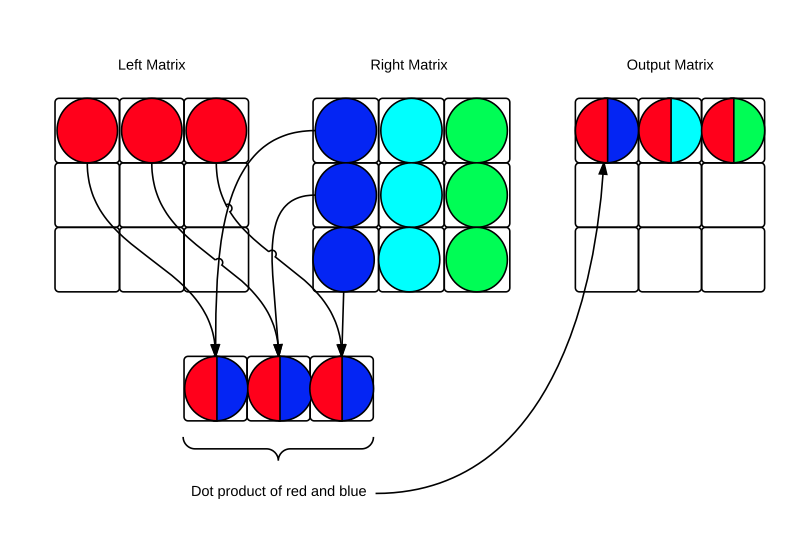
\includegraphics[scale = 0.4]{./matrix_mutiplication.png}
\caption{Standard matrix multiplication. The horizontal index of the left
    matrix and the vertical index of the right matrix are contracted away.
\label{fig:MatrixMultiplication}}
\end{figure}


Tensor contractions can be generalized to higher-dimension tensors, such as
three or four-dimensional tensors.

\section{Intrepid Contractions Overview}
Intrepid provides nine types of tensor contraction, differing by input
dimensionality, number of indices contracted away, and output dimensionality.
It is most simple to classify Intrepid's tensor contractions by number of
indices contracted away and output dimensionality.

Intrepid tensor contractions contract away one, two, or three indices. The
output of a single contraction can be a scalar (zero-dimensional), a vector
(one-dimensional), or a matrix (two-dimensional). Each combination of number of
contraction indices and output dimension is handled by one Intrepid tensor
contraction kernel.

\begin{table}[ht]
        \begin{tabular} {| l | l | l | l |l |}
            \hline
            \textbf{Kernel Name} & \textbf{Left Input} & \textbf{Right Input} &
            \textbf{Output} & \textbf{Contraction Indices}\\
            \hline
            ContractDataDataScalar   & 1D & 1D & Scalar & One \\
            ContractDataDataVector   & 2D & 2D & Scalar & Two \\
            ContractDataDataTensor   & 3D & 3D & Scalar & Three \\
            ContractDataFieldScalar  & 2D & 1D & Vector & One \\
            ContractDataFieldVector  & 3D & 2D & Vector & Two \\
            ContractDataFieldTensor  & 4D & 3D & Vector & Three \\
            ContractFieldFieldScalar & 2D & 2D & Matrix & One \\
            ContractFieldFieldVector & 3D & 3D & Matrix & Two \\
            ContractFieldFieldTensor & 4D & 4D & Matrix & Three \\
            \hline
        \end{tabular}
\caption{Summary of the nine Intrepid tensor contraction kernels
\label{tab:IntrepidContractionSummary}}
\end{table}

In order to more easily discuss specific tensor contraction kernels in Intrepid,
it helps to first understand the naming convention used for the kernel names.
Each kernel's name contains two suffixes, where the first indicates the
dimensionality of the output and the second indicates the number of contraction
indices.

\begin{table}[ht]
    \begin{center}
        \begin{tabular} {| l | l | l |}
            \hline
            \textbf{String} & \textbf{Position} & \textbf{Meaning} \\
            \hline
            DataData    & First Suffix  & Scalar Output    \\
            DataField   & First Suffix  & Vector Output    \\
            FieldField  & First Suffix  & Matrix Output    \\
            Scalar      & Second Suffix & One Contraction Index \\
            Vector      & Second Suffix & Two Contraction Indices \\
            Tensor      & Second Suffix & Three Contraction Indices \\
            \hline
        \end{tabular}
    \end{center}
\caption{Intrepid tensor contraction suffixes
\label{tab:IntrepidNamingConvention}}
\end{table}

For instance, in the \texttt{ContractDataDataScalar} kernel, the first suffix
\texttt{DataData} is used for kernels that produce scalar outputs, and the
second suffix \texttt{Scalar} is used for kernels that contract away one
dimension. Therefore, the Intrepid kernel \texttt{ContractDataDataScalar}
produces scalar outputs and contracts away one dimension, and so by necessity
the inputs for a single contraction must be vectors. All of the Intrepid tensor
contraction kernel suffixes are summarized in
Table~\ref{tab:IntrepidNamingConvention}. The nine tensor contractions in
Intrepid are summarized in Table~\ref{tab:IntrepidContractionSummary}.

Note that the tensor contraction kernels in Intrepid each actually performs many
contractions; for instance, \texttt{ContractDataDataScalar}, which performs
contractions of two input vectors to a single output scalar (dot product),
actually calculates an array of dot products. That is, the inputs are both
arrays of vectors, and the output is an array of scalars. This is represented
in the code using a dummy index, which we call the \texttt{Cell} index.

\section{ContractDataDataScalar}
\texttt{ContractDataDataScalar} is the simplest tensor contraction in Intrepid.
The kernel takes two arrays of vectors and outputs an array of scalars. A
snippet showing the simple serial implementation of
\texttt{ContractDataDataScalar} can be seen in
Figure~\ref{lst:ContractDataDataScalarSerial}.

\begin{figure}[ht]
    \begin{lstlisting}
    for (int c = 0; c < numCells; ++c) {
      for (int qp = 0; qp < quadraturePoints; ++qp) {
        output[c] += leftInput[c][qp] * rightInput[c][qp];
      }
    }
    \end{lstlisting}
\caption{Code from serial \texttt{ContractDataDataScalar}
\label{lst:ContractDataDataScalarSerial}} 
\end{figure}

As shown in 
Figure~\ref{lst:ContractDataDataScalarSerial}, this kernel contracts away the
\texttt{Quadrature Points} dimension, leaving only the \texttt{Cell} dimension.
It can also be thought of as an array of dot products.

\section{ContractDataDataVector}
\texttt{ContractDataDataVector} takes two arrays of two-dimensional tensors
(matrices) and computes an array of their inner products.
\begin{figure}[ht]
    \begin{lstlisting}
    for (int c = 0; c < numCells; ++c) {
      for (int qp = 0; qp < quadraturePoints; ++qp) {
        for (int t = 0; t < iVec; ++t) {
          output[c] += leftInput[c][qp][t] * rightInput[c][qp][t];
        }
      }
    }
    \end{lstlisting}
\caption{Code from serial \texttt{ContractDataDataVector}
\label{lst:ContractDataDataVectorSerial}} 
\end{figure}

As shown in Figure~\ref{lst:ContractDataDataVectorSerial},
\texttt{ContractDataDataVector} is very similar to
\texttt{ContractDataDataScalar}, except it contracts two indices instead of
one.

\section{ContractDataDataTensor}\label{section:ContractDataDataTensor}
\texttt{ContractDataDataTensor} takes two arrays of three-dimensional tensors
and computes an array of their inner products.

\begin{figure}[ht]
    \begin{lstlisting}
    for (int c = 0; c < numCells; ++c) {
      for (int qp = 0; qp < quadraturePoints; ++qp) {
        for (int t1 = 0; t1 < iVec1; ++t1) {
          for (int t2 = 0; t2 < iVec2; ++t2) {
            output[c] += leftInput[c][qp][t1][t2] * 
                         rightInput[c][qp][t1][t2];
          }
        }
      }
    }
    \end{lstlisting}
\caption{Code from serial \texttt{ContractDataDataTensor}
\label{lst:ContractDataDataTensorSerial}} 
\end{figure}

As shown in Figure~\ref{lst:ContractDataDataTensorSerial},
\texttt{ContractDataDataTensor} is very similar to\\
\texttt{ContractDataDataVector} and \texttt{ContractDataDataScalar}, but has
three contraction indices.

\section{ContractDataFieldScalar}

\texttt{ContractDataFieldScalar} takes an array of matrices and an array of
vectors and contracts away one index.

\begin{figure}[ht]
    \begin{lstlisting}
    for (int c = 0; c < numcells; ++c) {
      for (int l = 0; l < lbf; ++l) {
        for (int qp = 0; qp < quadraturepoints; ++qp) {
          output[c][l] += left[c][l][qp] * right[c][qp];
        }
      }
    }
    \end{lstlisting}
\caption{Code from serial \texttt{ContractDataFieldScalar}
\label{lst:ContractDataFieldScalarSerial}} 
\end{figure}

As shown in Figure~\ref{lst:ContractDataFieldScalarSerial},
\texttt{ContractDataFieldScalar} has two non-contraction indices, the
\texttt{Left Basis Function} index and the dummy \texttt{Cell} index. The
output for this contraction is therefore an array of vectors instead of an array
of scalars.

\section{ContractDataFieldVector}
\texttt{ContractDataFieldVector} takes an array of three-dimensional tensors and
an array of vectors, and contracts away two indices to produce an array of
vectors.

\begin{figure}[ht]
    \begin{lstlisting}
    for (int c = 0; c < numcells; ++c) {
      for (int l = 0; l < lbf; ++l) {
        for (int qp = 0; qp < quadraturepoints; ++qp) {
          for (int t = 0; t < iVec; ++t) {
            output[c][l] += left[c][l][qp][t] * right[c][qp][t];
          }
        }
      }
    }
    \end{lstlisting}
\caption{Code from serial \texttt{ContractDataFieldVector}
\label{lst:ContractDataFieldVectorSerial}} 
\end{figure}

As shown in Figure~\ref{lst:ContractDataFieldVectorSerial},
\texttt{ContractDataFieldVector} is similar to \texttt{ContractDataFieldScalar},
but has two contraction indices. 

\section{ContractDataFieldTensor}
\texttt{ContractDataFieldTensor} takes an array of four-dimensional tensors and
an array of three-dimensional tensors, and contracts away two indices to produce
an array of vectors.

\begin{figure}[ht]
    \begin{lstlisting}
    for (int c = 0; c < numcells; ++c) {
      for (int l = 0; l < lbf; ++l) {
        for (int qp = 0; qp < quadraturepoints; ++qp) {
          for (int t1 = 0; t1 < iVec1; ++t1) {
            for (int t2 = 0; t2 < iVec2; ++t2) {
              output[c][l] += left[c][l][qp][t1][t2] * right[c][qp][t1][t2];
            }
          }
        }
      }
    }
    \end{lstlisting}
\caption{Code from serial \texttt{ContractDataFieldTensor}
\label{lst:ContractDataFieldTensorSerial}} 
\end{figure}

As shown in Figure~\ref{lst:ContractDataFieldTensorSerial},
\texttt{ContractDataFieldTensor} is similar to \texttt{ContractDataFieldScalar},
but has three contraction indices. 

\section{ContractFieldFieldScalar}
\texttt{ContractFieldFieldScalar} takes in two arrays of matrices and performs
matrix multiplication on each element, yielding an output array of matrices.

\begin{figure}[ht]
    \begin{lstlisting}
    for (int c = 0; c < numcells; ++c) {
      for (int l = 0; l < lbf; ++l) {
        for (int r = 0; r < rbf; ++r) {
          for (int qp = 0; qp < quadraturepoints; ++qp) {
            output[c][l][r] += left[c][l][qp] * right[c][r][qp];
          }
        }
      }
    }
    \end{lstlisting}
\caption{Code from serial \texttt{ContractFieldFieldScalar}
\label{lst:ContractFieldFieldScalarSerial}} 
\end{figure}

As shown in Figure~\ref{lst:ContractFieldFieldScalarSerial},
\texttt{ContractFieldFieldScalar} has two non-contraction indices, so the output
is an array of matrices.

\section{ContractFieldFieldVector}
\texttt{ContractFieldFieldVector} takes two arrays of three-dimensional tensors
and contracts away two indices, keeping the \texttt{Cell} dummy dimension as
well as the left and right basis function indices.

\begin{figure}[ht]
    \begin{lstlisting}
    for (int c = 0; c < numcells; ++c) {
      for (int l = 0; l < lbf; ++l) {
        for (int r = 0; r < rbf; ++r) {
          for (int qp = 0; qp < quadraturepoints; ++qp) {
            for (int t = 0; t < iVec; ++t) {
              output[c][l][r] += left[c][l][qp][t] * right[c][r][qp][t];
            }
          }
        }
      }
    }
    \end{lstlisting}
\caption{Code from serial \texttt{ContractFieldFieldVector}
\label{lst:ContractFieldFieldVectorSerial}} 
\end{figure}

As shown in Figure~\ref{lst:ContractFieldFieldVectorSerial},
\texttt{ContractFieldFieldVector} is similar to
\texttt{ContractFieldFieldScalar}, but with two contraction indices.

\section{ContractFieldFieldTensor}
\texttt{ContractFieldFieldTensor} is the most complex of the tensor contraction
kernels in Intrepid. This kernel takes two four-dimensional tensors and
and contracts away three indices, keeping the \texttt{Cell} dummy dimension as
well as the left and right basis function indices.

\begin{figure}[ht]
    \begin{lstlisting}
    for (int c = 0; c < numcells; ++c) {
      for (int l = 0; l < lbf; ++l) {
        for (int r = 0; r < rbf; ++r) {
          for (int qp = 0; qp < quadraturepoints; ++qp) {
            for (int t1 = 0; t1 < iVec1; ++t1) {
              for (int t2 = 0; t2 < iVec2; ++t2) {
                  output[c][l][r] += left[c][l][r][qp][t1][t2] *
                  right[c][l][r][qp][t1][t2];
              }
            }
          }
        }
      }
    }
    \end{lstlisting}
\caption{Code from serial \texttt{ContractFieldFieldTensor}
\label{lst:ContractFieldFieldTensorSerial}} 
\end{figure}

As shown in Figure~\ref{lst:ContractFieldFieldTensorSerial},
\texttt{ContractFieldFieldTensor} is similar to
\texttt{ContractFieldFieldScalar}, but with two contraction indices.

        % ellen
    % Tensor Contractions in general
    % Intrepid specific contractions 
    % Serial snippets and descriptions

\chapter{Parallelism}

%Tyler
\section{Testing for Speedup}

Throughout our project, it was important to us to understand how performant our
code was compared to the existing code in Intrepid.  To do so, our team ran
performance testing using a machine equipped with an Intel\textsuperscript{\textregistered} Xeon\textsuperscript{\textregistered} E5-2630 v2
@ 2.60GHz CPU for our serial, OpenMP and Kokkos OpenMP testing and an NVIDIA 
Tesla K20m GPU for our Cuda and Kokkos GPU timing
testing. 

In order to generate plots that help understand how our code performs, we
collected data for each of our functors.  For serial code
and OpenMP code, this simply meant getting the time\footnote{We use
\texttt{clock\_gettime} instead of the C++11 high resolution timers for compatibility with
nvcc} before the block of code, and then getting the difference in time after
the block of code. See Figure~\ref{lst:OMPTiming} for an example of this. For
Cuda or Kokkos code, we instead start the clock before the kernel launch or call
to \texttt{parallel\_for}, and stop the clock after a device synchronize, so
that we know our code has finished running.

\begin{figure}[ht]
    \begin{lstlisting}
    timespec tic;
    timespec toc;
    
    clock_gettime(CLOCK_MONOTONIC, &tic);
    
    for ...
    	for ...  // Do OpenMP or serial contraction
    
    clock_gettime(CLOCK_MONOTONIC, &toc);
 \end{lstlisting}
\caption{Example timing for Serial/OpenMP code}
\label{lst:OMPTiming}
\end{figure}

In order to smooth our data, we run our timing tests 10 times, and use the
average time over all 10 attempts in our results. This was necessary in order to
counteract non-determinism and noise, but also has the potential to lead to caching
effects causing later attempts to be faster. In order to minimize caching, in
between timing tests we run kernels on the CPU and GPU that load a bunch of
junk data into memory, and then access it for dummy sums until we are satisfied
that the cache is clean.  Pseudocode for this can be seen in
Figure~\ref{lst:repeats}.

\begin{figure}[ht]
\begin{lstlisting}
    Kokkos::deep_copy(copy data to GPU);
    elapsedTime = 0
    for (int repeatIndex = 0; repeatIndex < 10; ++repeatIndex) {
        tic = start timing

        Kokkos::parallel_for(..., KokkosFunctor);
        Kokkos::fence();

        toc = stop timing
        elapsedTime += toc - tic

        Kokkos::parallel_for(..., DummyKokkosFunctorToClearCache);
        Kokkos::fence();
    }
    elapsedTime /= 10;
    Kokkos::deep_copy(copy results back to CPU);
 \end{lstlisting}
\caption{Pseudocode of running repeats for timing}
\label{lst:repeats}
\end{figure}

In future sections, wherever a graph appears with a label along the lines of
``Speedup over serial,'' (see Figure~\ref{lst:ContractFieldFieldScalar speedup
over serial} as an example), the data was obtained using this testing method on
our computer. Speedup over serial means the time of the serial code divided by
the time of kernel in question, and so that a reported speedup of 2 corresponds
to our kernel running twice as fast as the pre-existing serial code.


% Brett
\section{Flat Parallelism}
In this section, we will discuss how to write `flat' parallel code using Kokkos.
Flat parallel code is code that does not use Kokkos' thread teams concept, which
means that flat parallel code does not make use of GPU shared memory or
intra-team reductions.  Flat parallel code can coordinate between threads with atomic
instructions, but this can have performance costs. These costs occur because
atomic fetch and add can cause a bottleneck if too many threads are trying to
write to the same memory location. Therefore, in \emph{flat} algorithms, each
thread knows its responsibility and does not have to interact with other
threads. In this section we will describe how to write high performing kernels
for both the CPU and GPU using this flat parallelism technique. We will also
describe some of its shortcomings and which other non-flat parallel algorithms
solve these issues.

Over the course of our project, we identified four main factors that affect
code's performance. These factors are: the thread count, the amount of work each
thread must do, memory access patterns, and how data is laid out in memory.  The
first two factors (thread count and work per thread) are linked and are
inversely proportional to one another. 

The thread count and work per thread are generally determined by how far you
decide to break down a problem. For example, in
\texttt{ContractFieldFieldScalar}, which performs many matrix multiplications, a
programmer could make each thread do one full matrix multiplication. In this
case, the thread count must be equal to the number of cells, or matrix
multiplications, that must be calculated. Figuring out the best way to break
down the responsibility of a single thread requires looking at the expected
problem size. 

Representative use cases for \texttt{ContractFieldFieldScalar}
have from one thousand to tens of thousands of cells, with matrix sizes between
eight by eight and sixty-four by one hundred twenty-five. In this case, when
writing code for the GPU, it is best to break down the problem into the smallest
possible pieces that avoid interaction, which corresponds to one thread per
output element in each output matrix. This is because the goal is to minimize
the amount of work per thread on the GPU, while still avoiding thread
interaction. 

The question always becomes: how many threads per contraction is optimal?  As we
can see from the dimensions described above, our total number of threads will be
roughly 1,000 times our number of threads per contraction. Therefore, we would
like to have between a couple hundred and a thousand threads per contraction.
This will ensure that the GPU is being saturated, which is a necessary condition
for high performance.  To reiterate Section~\ref{CPU-GPU}, we need to make sure
that the GPU always has a \emph{minimum} of 15,000 threads being spawned, with
numbers in the 100,000-1,000,000 range being preferable.

When we combine this knowledge with the goal of the threads not being required
to interact or write to the same memory location, we discover that the ideal
number of threads per contraction we can use for flat parallelism is always the
same as the maximum number of threads we can use per contraction, because this
maximizes thread count and minimizes the work per thread.  The maximum number of
threads we can use is equal to of entries in the output tensor, because if we go
over that number, then the threads would need to interact to write to the same
output location.

Note that within the context of using Intrepid for finite element calculations,
the expected output tensor dimensions range from a single number (for any
problem that contains \texttt{DataData} in its name), to sixty-four squared (the
largest practical value for \texttt{numLeftFields} and \texttt{numRightFields},
which are the dimensions of the output matrix for some problems). This range
means that if we use flat parallelism for the \texttt{DataData} contractions, we
will only be spawning 1,000-10,000 threads on the GPU in the normal use cases,
which are below acceptable in terms of saturation.  Figure~\ref{fig:CDDT2d}
illustrates this effect.

\begin{figure}[!ht]
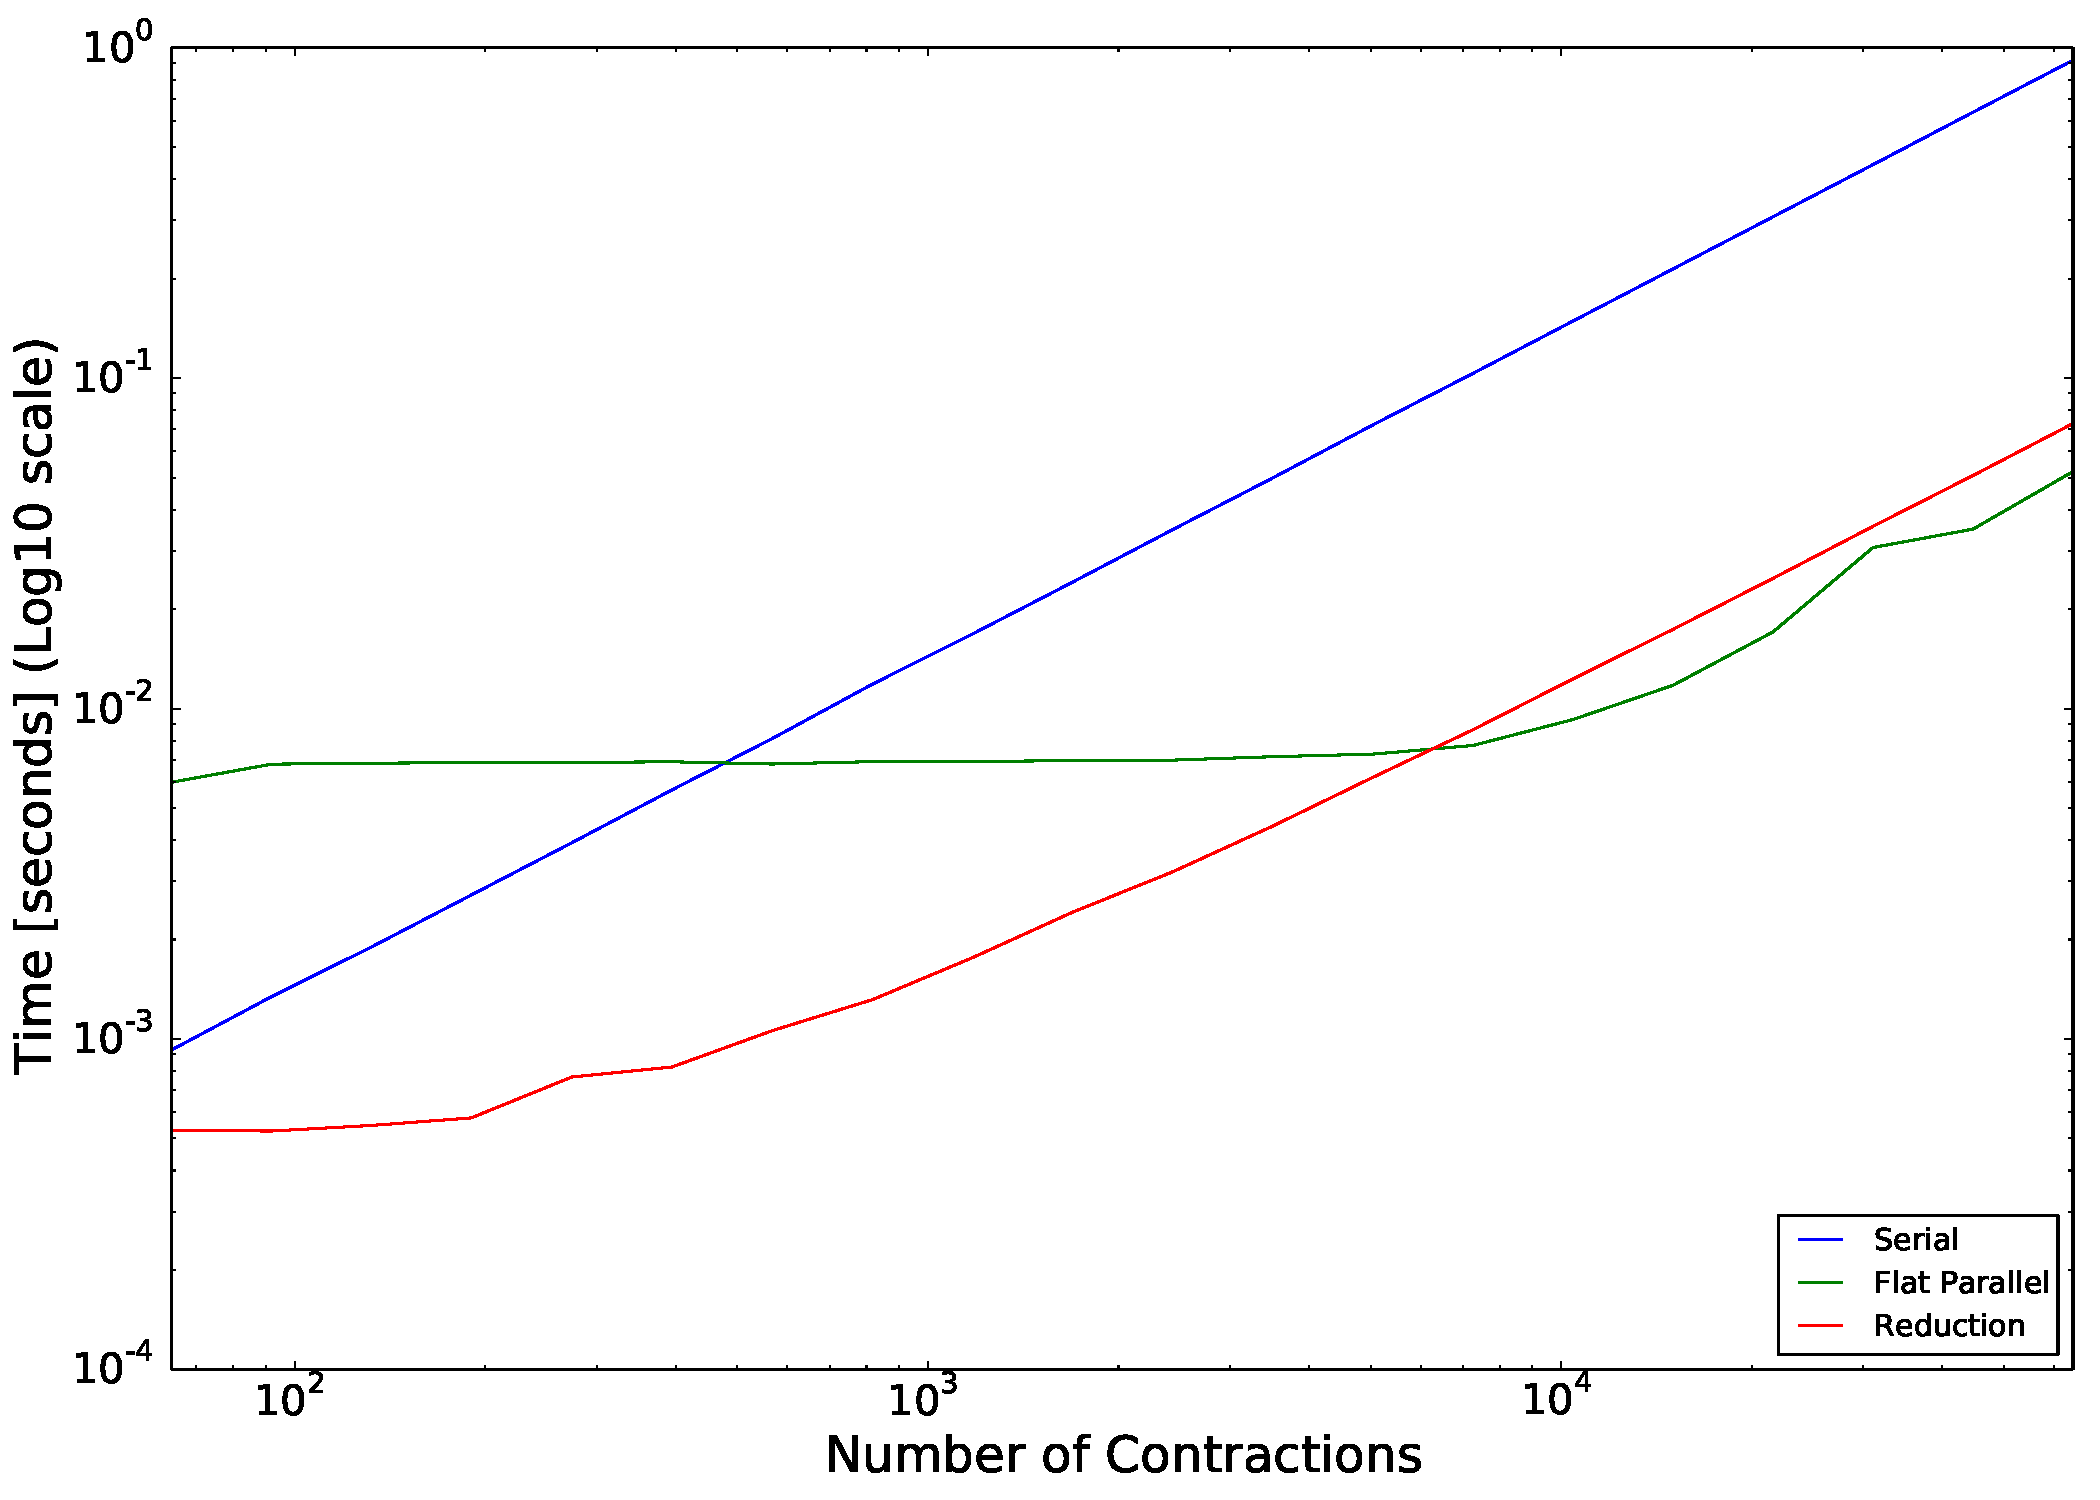
\includegraphics[width=5in]{CDDT2D}
\caption[\texttt{ContractDataDataTensor} performance 2d summary]{Performance of
\texttt{ContractDataDataTensor} flat parallel, serial, and reduction algorithms.
The reduction algorithm used here is the Teamstride algorithm, detailed in
Section~\ref{sec:Teamstride}}
\label{fig:CDDT2d} 
\end{figure}

Now that the number of threads and their responsibility are known, the best
access patterns and data layouts must be determined. As described earlier, the
best access patterns and data layouts for threads on the CPU are ones that
utilize the cache. This means that when using CPU, which corresponds to code
written with \texttt{Kokkos::OpenMP}, we want a thread's next memory read to be
next to its current memory read.  However, when using the GPU, which corresponds
to code written with \texttt{Kokkos::Cuda}, a thread's memory read should be
adjacent to the reads of threads with nearby indices, as these threads will be
in the same warp. 

These two memory access patterns are in direct conflict. To solve this problem,
Kokkos abstracts out the data layout by introducing a data structure called a
\texttt{View} that encodes multidimensional arrays with custom memory layouts. The main
layout parameters to a Kokkos View are \texttt{LayoutLeft} and
\texttt{LayoutRight}. In \texttt{LayoutLeft}, the left-most indices are adjacent
in memory, i.e., incrementing the left-most index by 1 moves to the next memory
location.  The opposite is true for \texttt{LayoutRight}.  This means we can use
\texttt{LayoutLeft} for one architecture, (i.e.  \texttt{Kokkos::Cuda}), and
\texttt{LayoutRight} for the other (\texttt{Kokkos::OpenMP}) \footnote{In fact,
if the memory layout for a view is not provided, Kokkos will default to
\texttt{LayoutLeft} on the GPU and \texttt{LayoutRight} on a CPU}. 

All that remains is to figure out how to arrange the data, or which order to put
the indices so that one layout coalesces the memory while the other uses the
cache. This is best shown by an example; in \texttt{ContractFieldFieldScalar}
there are inputs $A_{c, l, p}$ and $B_{c, r, p}$. Assuming we have a thread per
output element in output $C_{c, l, r}$, then we can have the inputs ordered as
follows: $A_{c, l, p}$ and $B_{c, r, p}$. When using \texttt{Kokkos::OpenMP}, we
will assume that the Views are \texttt{LayoutRight}, so $A_{i, j, k}$ will be
right next to $A_{i, j, k+1}$ in memory, while $A_{i, j, k}$ will be very far
from $A_{i+1, j, k}$ in memory. Each thread needs to do a dot product of a row
in $A$ with a column in $B$, so a thread needs to loop through all of $p$ for
the same value of $c$ and $l$ in $A$ and also loop through all of $p$ for the
same $c$ and $r$ in $B$. Notice however that all the different values of $p$ in
$A$ and $B$, where $c$, $l$, and $r$ are fixed, are next to each other in
memory, since we are using \texttt{LayoutRight}. This means that it will be
cache friendly for any thread. 

In contrast, for \texttt{Kokkos::Cuda}, the memory accesses must be coalesced in
the optimal case.  This can be achieved by using the same data, but storing it
in \texttt{LayoutLeft} Views instead of \texttt{LayoutRight} Views. In this
case, $c$ values that differ by 1 are adjacent in memory.  Therefore, if thread
$x$ is responsible for calculating $C_{i, j, k}$, thread $x+1$ should
responsible for calculating $C_{i+1, j, k}$. In this manner, by changing our
threading policy and the layout of our Views, our memory accesses are now
coalesced, as desired. 

Finding the best way to lay out memory to optimize for both the CPU and GPU is
not too difficult. One good technique is to first find the best way for caching (CPU),
then imagine using the opposite layout (left or right) and check if there is
any way to coalesce the memory. This way one functor can be used, the data
layout can be easily changed, and the performance for both the CPU and GPU will
be high. Using this flat parallel technique we have achieved many good results,
an example of which can be seen in Figure~\ref{lst:ContractFieldFieldScalar
speedup over serial}

It is important to find a way to arrange the indices of the data such that
caching and coalescing can be achieved by changing the layout of the View (as we
just did).  Laying out the data correctly allows threading policies for both the
CPU and the GPU to match the data layout.  This is impossible or difficult with
a bad data layout, forcing the developer to write different code for
different architectures, which is undesirable.

\begin{figure}[!ht]
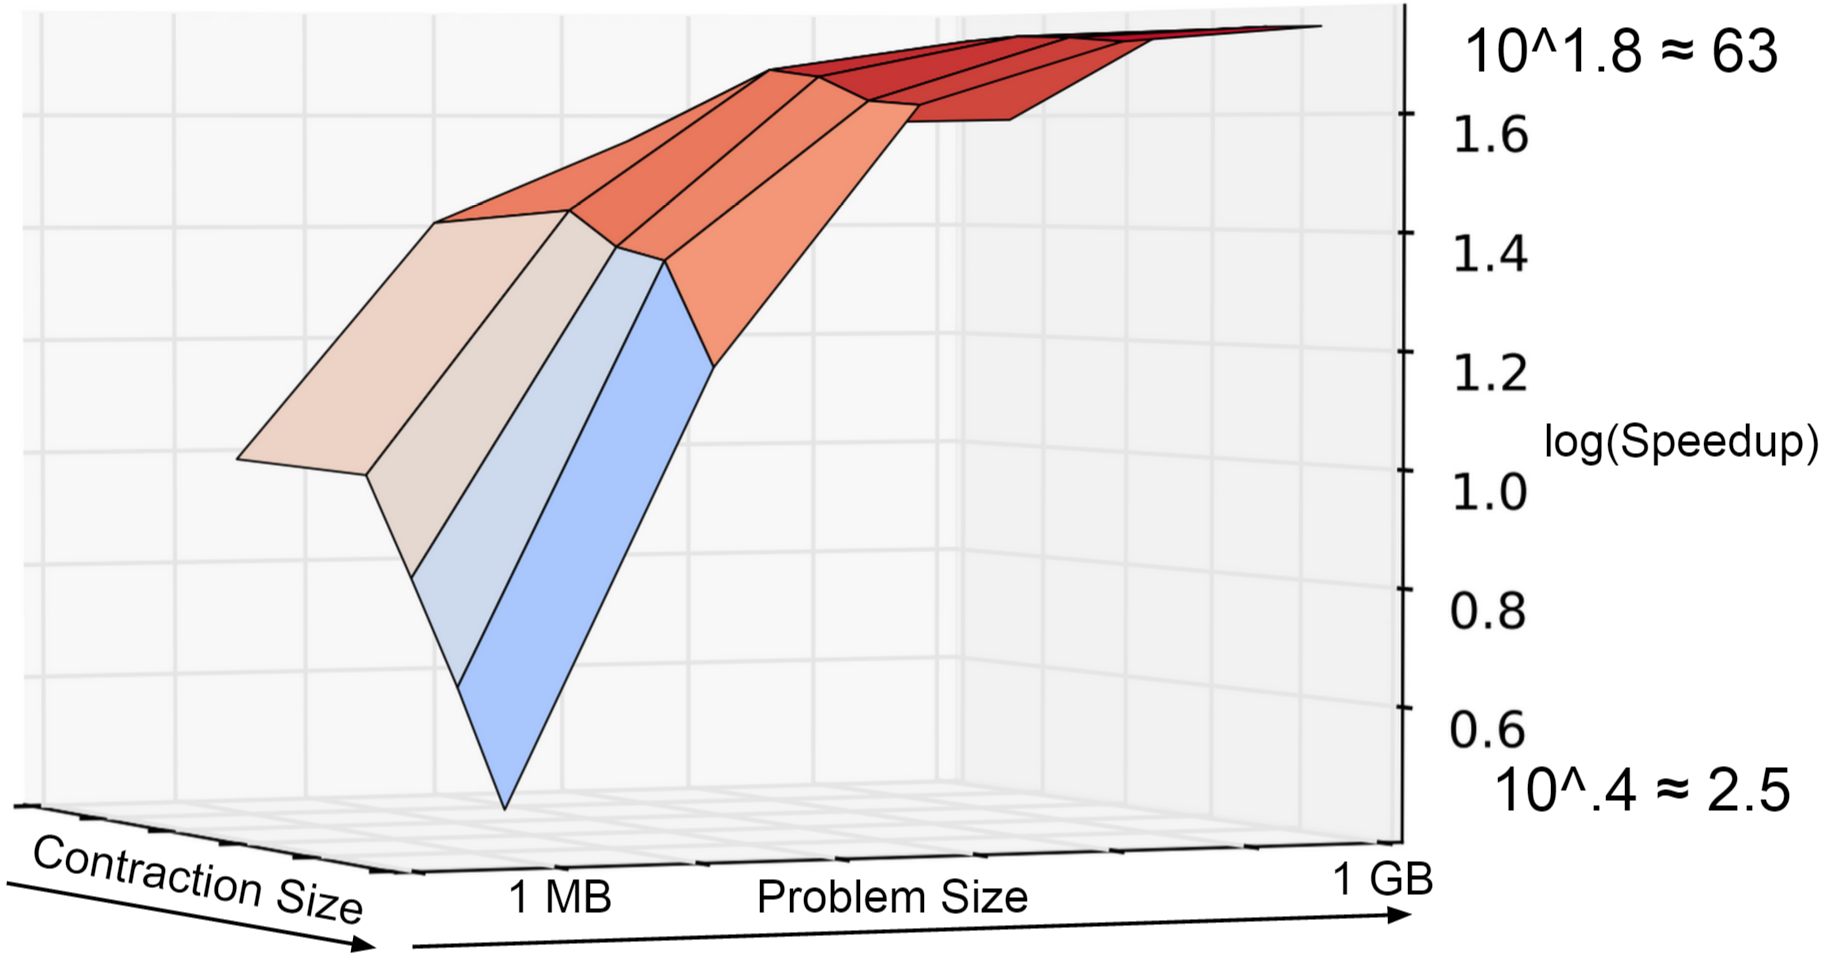
\includegraphics[width=5in]{CFFSIndependent2.PNG}
\caption[Performance of \texttt{ContractFieldFieldScalar} flat parallel]
{Speedup over serial of the flat parallel algorithm of the
\texttt{ContractFieldFieldScalar} kernel. At its best this algorithm runs 60
times faster than serial. The closest corner, where speedup is only about 2.5
times, does not fit into Sandia's use case of expected problem sizes.
\label{lst:ContractFieldFieldScalar speedup over serial}} 
\end{figure}

Flat parallelism is an easy-to-implement, high-performing algorithm when there
is enough work to saturate the GPU. However, there isn't always enough
independent work to use flat parallelism. For example, on all the problems that
have \texttt{DataData} in their name, the output is simply an array of scalars,
meaning that only one thread per contraction can be used. The GPU is great for
using tens of thousands of threads to do computation, but when the number of
threads is severely limited, the CPU performs better, so other algorithms must
be explored on the GPU.  For examples of these algorithms, see
Section~\ref{sec:reduction}

Another feature of the GPU that cannot be used by flat parallelism algorithms in
Kokkos is shared memory. Shared memory is essentially a user controlled cache on
the GPU.  Algorithms that use shared memory will be discussed in
Section~\ref{sec:Slicing} and Section~\ref{sec:tiling}. The main benefits of not
using shared memory are it is easier to code and the speedup of shared memory
over flat parallelism is relatively small compared to the speedup flat parallel
algorithms reap over serial code. 

% Ellen
\section{Reduction} \label{sec:reduction}
In some cases, flat parallelism can perform very poorly.  One problem with flat
parallelism is the potential lack of enough parallelism, as in
\texttt{ContractDataDataTensor}.  \texttt{ContractDataDataTensor} takes two
input arrays of three-dimensional tensors and produces an array of scalars.  See
Section~\ref{section:ContractDataDataTensor} for a more complete description of
this kernel.

The problem with the \texttt{DataData} class of tensor contractions (see
Table~\ref{tab:IntrepidNamingConvention}) is that they all output an array of
scalars -- that is, each individual contraction produces a scalar output.
Therefore, using flat parallelism, the greatest number of threads we can spawn
is one thread per contraction.  Each thread must then perform an entire
contraction independently, which in the case of
\texttt{ContractDataDataTensor}, means looping over all three of the
contraction indices.

Because of this, we see that when the contraction size is large and the memory
size is small -- when we cannot spawn enough threads to saturate the GPU and
each thread is responsible for a large amount of computation --
\texttt{ContractDataDataTensor} actually performs worse than serial, as seen in
Figure~\ref{fig:CDDT2d}.

A solution to this problem is to use a parallel reduction algorithm instead of
a flat parallelism algorithm.  In a reduction, multiple threads contribute to a
single output element.  This adds the necessary overhead of coordinating between
threads and combining their contributions, but allows more threads to be created
to saturate the GPU.

In Kokkos, threads can be organized into teams\footnote{for seasoned Cuda
programmers, teams correspond to Cuda blocks}.  Built-in reduction methods allow
teams to merge the contributions of their constituent threads.
Using this team-thread paradigm, we explored several methods of implementing
\texttt{ContractDataDataTensor} using a reduction algorithm.

\subsection{Team Depth 1}
    In this reduction algorithm, we assign one team per contraction, and each
    team has as many threads as there are elements in the \texttt{\_dim2}
    dimension.  Each thread therefore performs 
    $\texttt{\_numPoints} \times \texttt{\_dim1}$ multiplications, and then
    combines its local sum with that
    of the other threads in the team.


\begin{figure}[ht]
    \begin{lstlisting}[basicstyle=\tiny]
    // A team does one cell
    const unsigned int cellIndex = thread.league_rank();

    float sum = 0;
    
    // Each of the _dim2 threads contracts the qp and d1 dimensions.  All of the
    // Views are layout right; d2 is stride 1.  This is coalesced, but not
    // cached for the CPU.
    Kokkos::parallel_reduce(Kokkos::TeamThreadLoop(thread, _dim2),
    // We use an anonymous (lambda) function here:
    //      - [&] specifies that all automatic variables in the lambda are
    //         passed by reference; this allows us to save time that would be
    //         spent copying large arrays.
    //      - The lambda takes two arguments, d2 by value and localsum by
    //         reference.  The first argument is passed to each thread (this is
    //         the index into the _dim2 dimension to be looped over by this
    //         thread), and the second is the reduction target.
        [&] (const unsigned int d2, float& localsum) {
          for (unsigned int qp=0; qp < _numPoints; ++qp) {
            for (unsigned int d1=0; d1 < _dim1; ++d1) {
              // Each thread loops over two dimensions and then reduces into
              // localsum
              localsum +=  _leftInput(cellIndex, qp, d1, d2) *
                _rightInput(cellIndex, qp, d1, d2);
            }
          }
      }, sum);

    if (thread.team_rank() == 0) {
      _output(cellIndex) = sum;
    }
 \end{lstlisting}
\caption{\texttt{ContractDataDataTensor} Team Depth 1 functor
\label{lst:ContractDataDataTensorDepth1Functor}} 
\end{figure}

\begin{figure}[ht]
    \begin{lstlisting}
    const team_policy reduction_policy(numCells, _dim2);
    Kokkos::parallel_for(reduction_policy, contractDataDataTensorTeamDepth1Functor );
    Kokkos::fence();
 \end{lstlisting}
\caption{\texttt{ContractDataDataTensor} Team Depth 1 kernel launch
\label{lst:ContractDataDataTensorDepth1Call}} 
\end{figure}

In Figure~\ref{lst:ContractDataDataTensorDepth1Functor}, we can see that each
thread loops over the \texttt{\_numPoints} and \texttt{\_dim1} dimensions, and then
reduces with the other threads in the team.  The call to Kokkos'
\texttt{parallel\_for} function, seen in
Figure~\ref{lst:ContractDataDataTensorDepth1Call}, specifies an execution policy
in which the number of teams launched is \texttt{\_numCells}, and each team has
\texttt{\_dim2} threads.

\begin{figure}[ht]
    \begin{centering}
    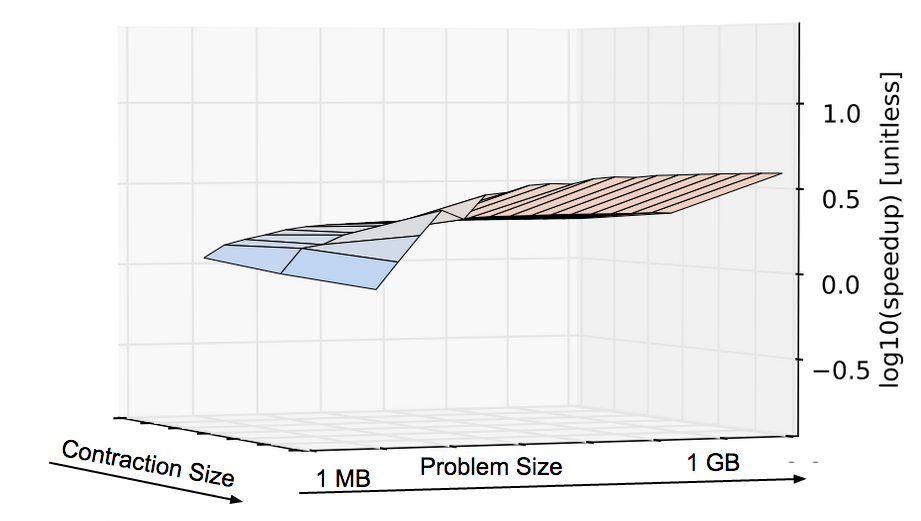
\includegraphics[width=5in]{./VersusSerial_kokkosCudaTeamDepth1_clearCache_shadowfax}
\end{centering}
    \caption[Performance of \texttt{ContractDataDataTensor} Team Depth
    1]{Speedup of \texttt{ContractDataDataTensor} Team Depth 1 reduction over
    serial
\label{fig:ContractDataDataTensorDepth1}} 
\end{figure}

As shown in Figure~\ref{fig:ContractDataDataTensorDepth1}, this Team Depth 1
algorithm performs generally better than serial, but the speedup is minimal.
Therefore, we explored other reduction algorithms, which we hoped would yield
more impressive results.

\subsection{Team Depth 2}
    This reduction algorithm is similar to the previous one.  In a similar
    approach to that taken in the Team Depth 1 reduction, we assign one team per
    contraction.  In contrast to Team Depth 1, here each team has
    $\texttt{\_dim1} \times \texttt{\_dim2}$ threads, each responsible for
    \texttt{\_numPoints} multiplications.  Each thread then combines its local
    sum with that of the other threads in the team.

\begin{figure}[ht]
    \begin{lstlisting}
    // A team does one cell
    const unsigned int cellIndex = thread.league_rank();

    float sum = 0;
    // Each of the _dim1 * _dim2 threads contracts the _numPoints dimension
    Kokkos::parallel_reduce(Kokkos::TeamThreadLoop(thread, _dim1 * _dim2),
        [&] (const unsigned int threadIndex, float& localsum) {
          const unsigned int d1 = threadIndex / _dim2;
          const unsigned int d2 = threadIndex % _dim2;

          for (unsigned int qp = 0; qp < _numPoints; ++qp) {
            localsum +=  _leftInput(cellIndex, qp, d1, d2) *
              _rightInput(cellIndex, qp, d1, d2);
          }

      }, sum);

    if (thread.team_rank() == 0) {
      _output(cellIndex) = sum;
    }
    
 \end{lstlisting}
\caption{\texttt{ContractDataDataTensor} Team Depth 2 functor 
\label{lst:ContractDataDataTensorDepth2Functor}} 
\end{figure}

\begin{figure}[ht]
    \begin{lstlisting}
    const team_policy reduction_policy(numCells, _dim2 * _dim1);
    Kokkos::parallel_for(reduction_policy, contractDataDataTensorTeamDepth2Functor );
    Kokkos::fence();
 \end{lstlisting}
\caption{\texttt{ContractDataDataTensor} Team Depth 2 kernel launch
\label{lst:ContractDataDataTensorDepth2Call}} 
\end{figure}

In Figure~\ref{lst:ContractDataDataTensorDepth2Functor}, we can see that each
thread loops over the \texttt{\_numPoints} dimension only, and then
reduces with the other threads in the team.  The call to Kokkos'
\texttt{parallel\_for} function, seen in
Figure~\ref{lst:ContractDataDataTensorDepth2Call}, specifies an execution policy
in which the number of teams launched is \texttt{\_numCells}, and each team has
$\texttt{\_dim1}\times \texttt{\_dim2}$ threads.

\begin{figure}[ht]
    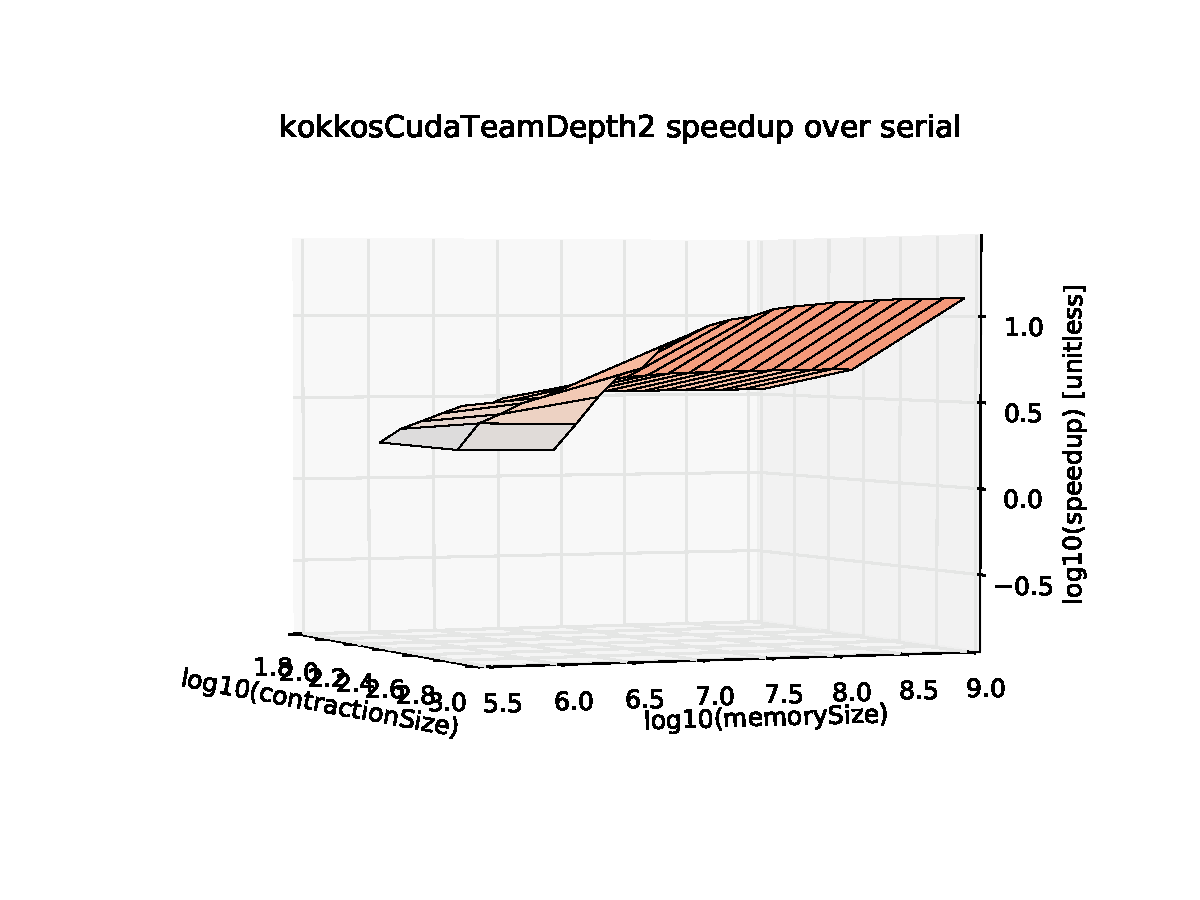
\includegraphics[width=5in]{./VersusSerial_kokkosCudaTeamDepth2_clearCache_shadowfax}
    \caption[Performance of \texttt{ContractDataDataTensor} Team Depth
    2]{Speedup of \texttt{ContractDataDataTensor} with Team Depth 2 reduction
    over serial
\label{fig:ContractDataDataTensorDepth2}} 
\end{figure}

As shown in Figure~\ref{fig:ContractDataDataTensorDepth2}, this Team Depth 2
algorithm performs better than serial for the three representative use case..
In addition, the speedup is significant, and for large memory sizes, performs
nearly as well as the flat parallel algorithm, as seen in
Figure~\ref{fig:CDDT2d}.  Given the necessary overhead of
performing a reduction, we believe this to be a fairly good algorithm for good
performance across the
board.

However, because the team size is fixed based on the size of the \texttt{\_dim1}
and \texttt{\_dim2} dimensions, this algorithm may suffer performance penalties
or perhaps even bugs if these two dimensions are of unexpected sizes.  A more
generalizable algorithm therefore would be preferable.

\subsection{Teamstride}\label{sec:Teamstride}
    A more robust algorithm is one we call the Teamstride algorithm, in which
    each contraction is still assigned to a team, but a fixed number of threads
    are spawned for each team.  These threads treat the three contraction
    indices (\texttt{\_numPoints}, \texttt{\_dim1}, \texttt{\_dim2}) as if they were
    a single index, each thread striding forwards by the number of threads on
    this ``combined'' index.  This technique is similar to that used by OpenMP's
    collapse clause.  For instance, if this algorithm were run with a team size
    of sixty-four threads, then the zeroth thread in a team would sum the
    product of the zeroth elements, the sixty-fourth, the 128th, and so on.
    
\begin{figure}[ht]
    \begin{lstlisting}
    // A team does one cell
    const unsigned int cellIndex = thread.league_rank();

    float sum = 0;

    Kokkos::parallel_reduce (Kokkos::TeamThreadLoop(thread,cellSize),
       [&](const unsigned int threadIndex, float& localsum) {
        // Calculate the next element to add (striding by teamsize)
        const unsigned int qp = threadIndex / (_dim1 * _dim2);
        const unsigned int d1 = threadIndex % (_dim1 * _dim2) / _dim2;
        const unsigned int d2 = threadIndex % _dim2;
        
        localsum +=  _leftInput(cellIndex, qp, d1, d2) *
          _rightInput(cellIndex, qp, d1, d2);
      } , sum );

    if (thread.team_rank() == 0) {
      _output(cellIndex) = sum;
    }
\end{lstlisting}
\caption{\texttt{ContractDataDataTensor} Teamstride functor
\label{lst:ContractDataDataTensorTeamstrideFunctor}} 
\end{figure}

\begin{figure}[ht]
    \begin{lstlisting}
    const team_policy reduction_policy(numCells, 32);
    Kokkos::parallel_for( reduction_policy, contractDataDataTensorTeamstrideFunctor );
    Kokkos::fence();
    \end{lstlisting}
\caption{\texttt{ContractDataDataTensor} Teamstride kernel launch
\label{lst:ContractDataDataTensorTeamstrideCall}} 
\end{figure}

As seen in Figure~\ref{lst:ContractDataDataTensorTeamstrideFunctor}, this
algorithm requires more arithmetic on the part of each thread because the thread
is not responsible for looping over a single subset of indices but is instead
looping over all three contraction indices. The corresponding call in
Figure~\ref{lst:ContractDataDataTensorTeamstrideCall} uses a fixed team size of
32, unlike the previous two algorithms.  This team size seemed to be the best
for performance; a team size of 64 yielded similar speedup, but larger team
sizes did not perform as well.

\begin{figure}[ht]
    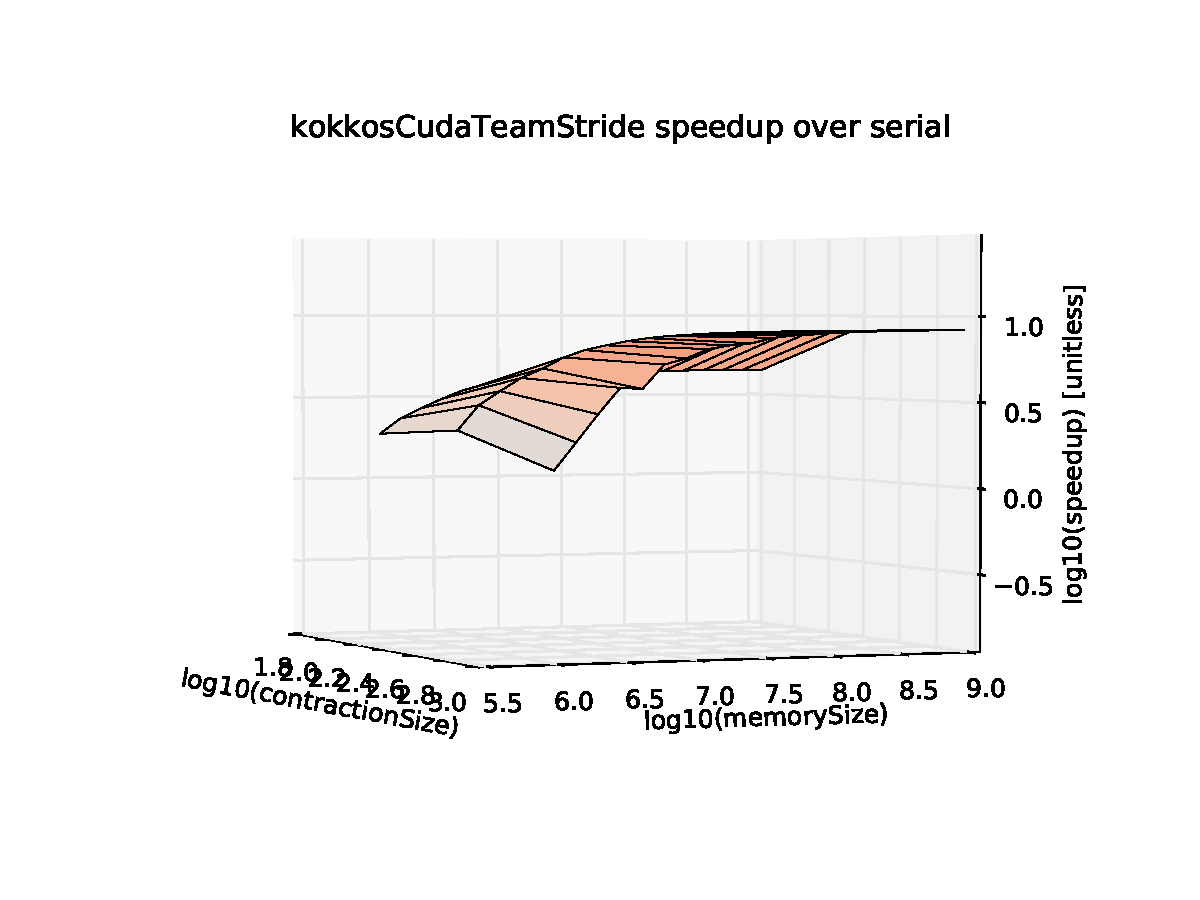
\includegraphics[width=5in]{./VersusSerial_kokkosCudaTeamStride_clearCache_shadowfax}
    \caption[Performance of \texttt{ContractDataDataTensor} Teamstride]{Speedup
        of \texttt{ContractDataDataTensor} with Teamstride algorithm over serial
\label{fig:ContractDataDataTensorTeamstride}} 
\end{figure}

As shown in Figure~\ref{fig:ContractDataDataTensorTeamstride}, this algorithm
always performs better than serial.  Like with Team Depth 2, the speedup is
significant, and for large memory sizes, performs nearly as well as the flat
parallel algorithm.  In addition, this algorithm is more robust than Team Depth
2, since the number of threads per team is not determined by the size of the
input dimensions.  Therefore, the Teamstride reduction algorithm is likely the
most generalizable and performant variant of the reduction algorithms, and
should be explored in tensor contraction functions in which the inputs may
consist of a few large tensor contractions.

\subsection{Reduction Special Case}
As mentioned above, the parallel reduction algorithm outperforms the flat
parallel algorithm when there is a small number of threads but a significant
amount of work per
thread. We also created parallel reduction algorithms for problems that did not
have this issue. An example is \texttt{ContractFieldFieldScalar}, which could have as
small as eight multiplies for a single thread since $p$ could be as few as
eight. As one may guess, the Teamstride parallel reduction algorithm performs
worse than the flat parallel algorithm. This is because we are creating more
threads than necessary and dividing up a small amount of work between at least
32 threads. The work is divided between at least 32 threads because, remembering
the architecture of the GPU, there are 32 threads in a warp, all of which run in
lockstep. So in cases where $p < 32$, threads are created that are not used in
this reduction algorithm. To mitigate this phenomenon we created a special
reduction case.

The special reduction case creates fewer teams, giving more work per team, if
more than half of the threads in a warp are being wasted. In
\texttt{ContractFieldFieldScalar}, where 24 threads can wasted because only
eight need to do a multiply then reduction, this special case creates one-fourth
as many teams, and each team is responsible for calculating four times as many
outputs elements.  This case adds the code in
Figure~\ref{lst:ContractFieldFieldScalarReductionSpecialCase} to the functor's
operator() function.

\begin{figure}[!ht]
    \begin{lstlisting}
// The if case is where the special reduction case is handled
if (numPoints <= 16) {	
	int myID = thread.league_rank()*(threadsPerTeam/numPoints)+thread.team_rank()/numPoints;
	int myMatrix = myID / (numLeftFields * numRightFields);
	int matrixIndex = myID - (myMatrix * (numLeftFields * numRightFields));
	int matrixRow = matrixIndex / numRightFields;
	int matrixCol = matrixIndex - (matrixRow * numRightFields);

	int pointIndex = thread.team_rank() % numPoints;

	float mult = leftView(myMatrix, matrixRow, pointIndex) 
		* rightView(myMatrix, pointIndex, matrixCol);

	Kokkos::atomic_fetch_add(&outputView(myMatrix, matrixRow, matrixCol), mult);
}
// This is where the normal reduction case is handled
else {
	int myID = thread.league_rank();
	int myMatrix = myID / (_numLeftFields * _numRightFields);
	int matrixIndex = myID - (myMatrix * (_numLeftFields * _numRightFields));
	int matrixRow = matrixIndex / _numRightFields;
	int matrixCol = matrixIndex - (matrixRow * _numRightFields);

	Kokkos::parallel_reduce(Kokkos::TeamThreadLoop(thread, _numPoints),
		[&] (const unsigned int& i, float& localSum) {
			localSum += _leftView(myMatrix, matrixRow, i) *
				_rightView(myMatrix, i, matrixCol);
			},
			sum);
	if (thread.team_rank() == 0) {
		_outputView(myMatrix, matrixRow, matrixCol) = sum;
	}
}
    \end{lstlisting}
\caption{Code for \texttt{ContractFieldFieldScalar} special reduction case
\label{lst:ContractFieldFieldScalarReductionSpecialCase}} 
\end{figure}

In the code of Figure~\ref{lst:ContractFieldFieldScalarReductionSpecialCase},
the number of multiplies that is needed is \texttt{numPoints}. If that number is less
than 16, then we want one team to do more than one output. Increasing the number
of active threads per team leads to higher efficiency and speed.  Note that the
special case uses an \texttt{atomic\_fetch\_add} a \texttt{parallel\_reduce}.
This is due to the fact that there is no \texttt{parallel\_reduce} function
where half the threads reduce to one location while the other half reduce to
another location. This has the side effect of requiring the output locations to
be zeroed out before the calculation, while in the "normal" reduction algorithm
that is not necessary. 

This special case can still
perform worse than the flat parallel algorithm, it does increase 
the performance of a pure reduction algorithm in the region of the plot where it
performs most poorly. Figure~\ref{CFFSTeamReduceSpecialCaseGraph} shows the
effect of using the special case. The ``flap up'' for small contraction sizes
does not exist for the algorithm not including the special case. The reduction
with the special case significanly outperforms the reduction algorithm without
the special case for small contraction sizes.

\begin{figure}
    \centering
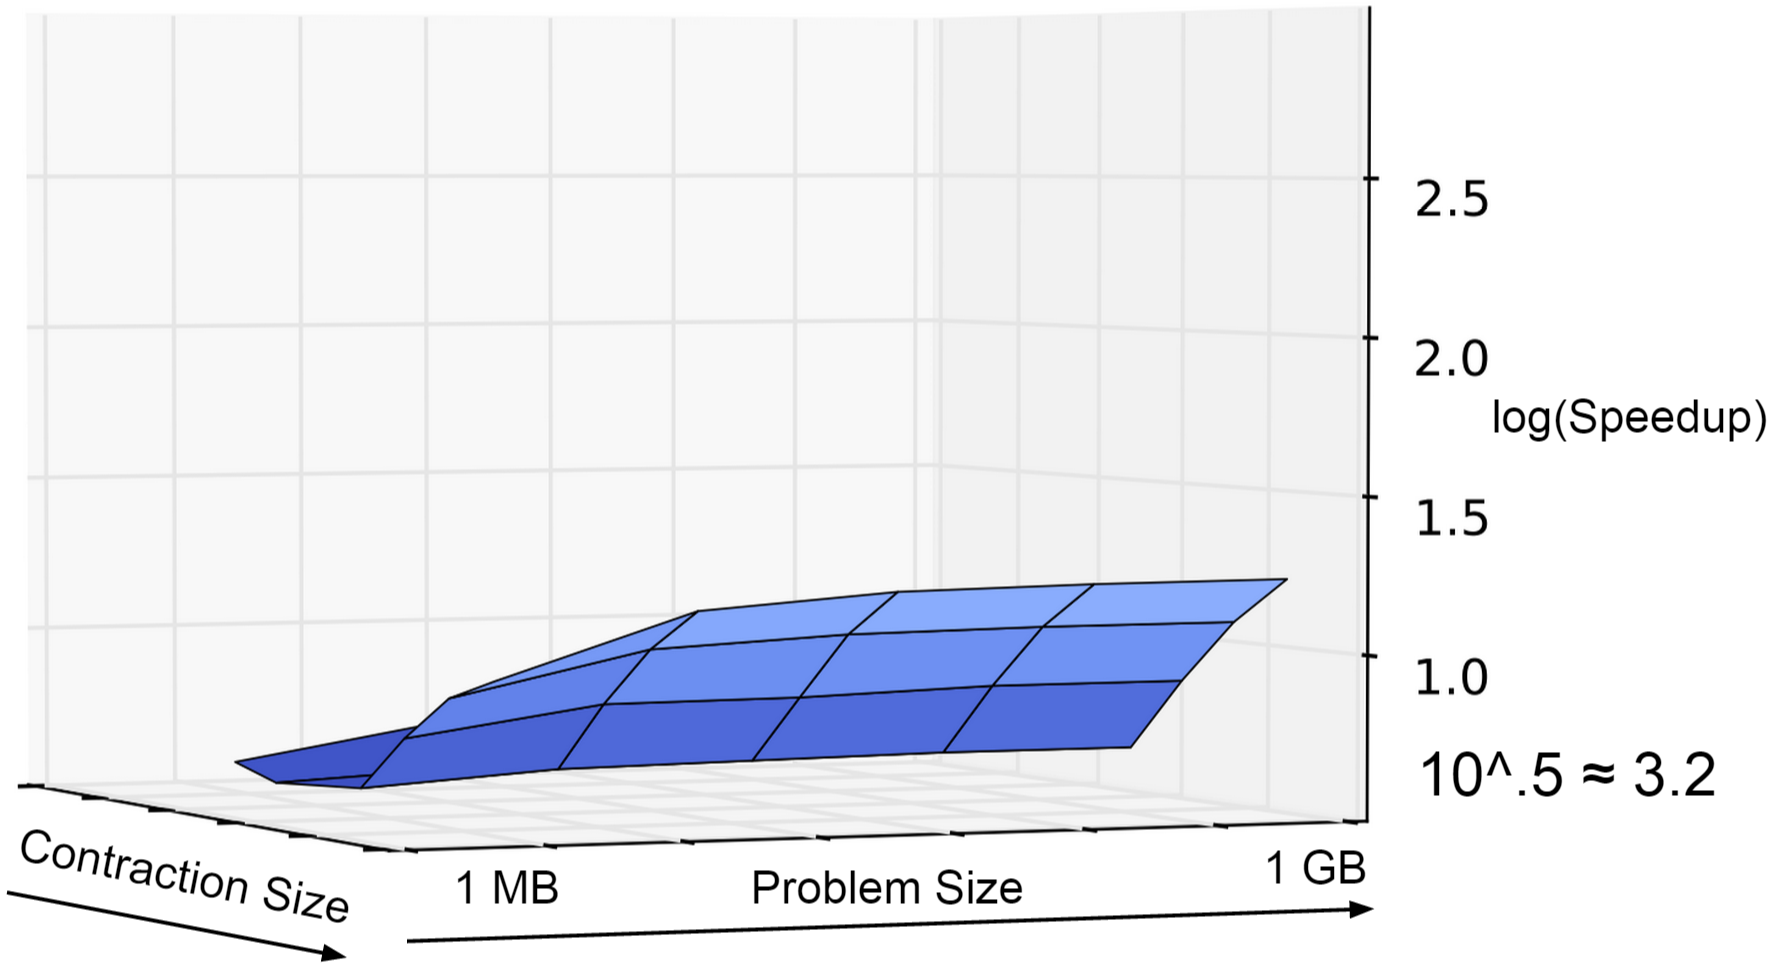
\includegraphics[width=5in]{ReductionSpecial2.png}
\caption[\texttt{ContractFieldFieldScalar} reduction special]{Graph showing the
    special case of Team Reduction algorithm's speedup over serial for
    \texttt{ContractFieldFieldScalar}.  The faster speeds for the smaller
contraction size (far left) is where the special case is used.}
\label{CFFSTeamReduceSpecialCaseGraph}
\end{figure}

\begin{figure}
    \centering
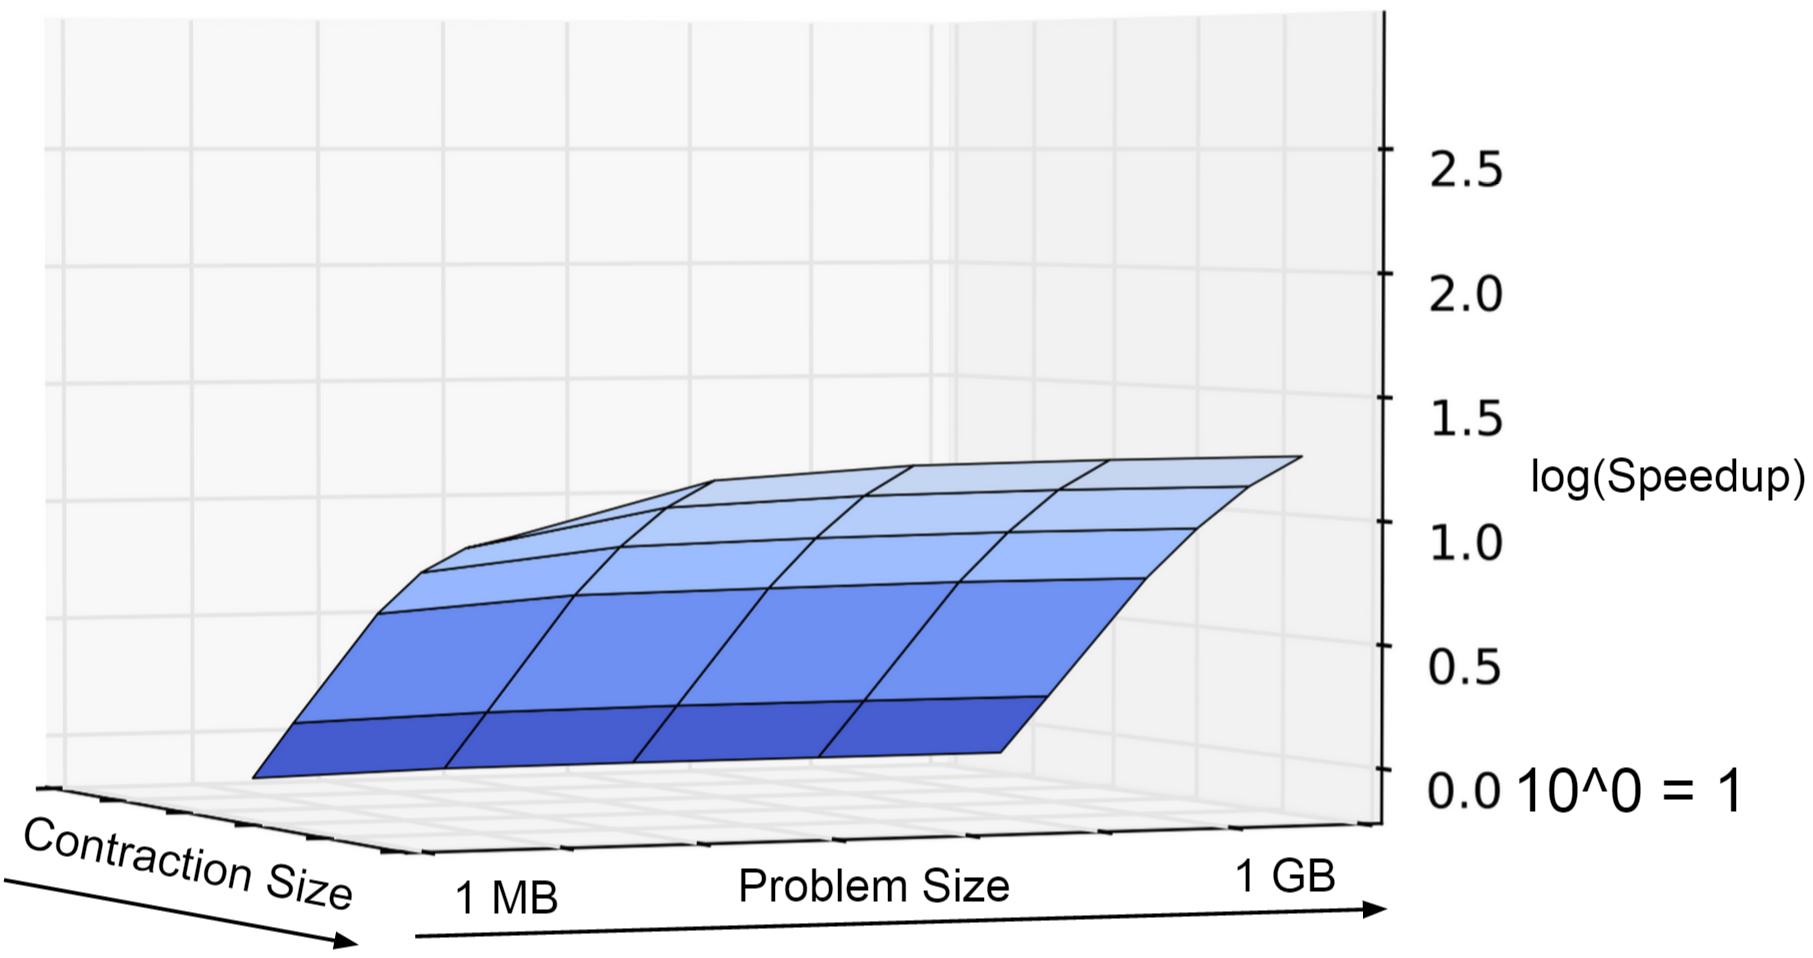
\includegraphics[width=5in]{ReductionNoSpecial2.png}
\caption[\texttt{ContractFieldFieldScalar} reduction no special]{\texttt{ContractFieldFieldScalar} team reduction's speedup
        over serial without the special case in the reduction. Notice that the
    smaller contraction sizes continue to perform worse, which was not the case
for the reduction algorithm with the special case.}
\label{CFFSTeamReduceNoSpecialCaseGraph}
\end{figure}

\subsection{A Note on Data Shape} \label{sec:DataShape}
In both of the next two approaches, we benchmarked our code using a different data layout than the native
Sandia code. For example, in \texttt{ContractFieldFieldScalar} our input matrices were placed in memory as $A_{c,l,p}$ and
$B_{c,p,r}$ instead of $A_{c,l,p}$ and $B_{c,r,p}$ (as they are arranged in the native Sandia code).
This means that the code we wrote would have to be changed to account for this different layout
before it could be integrated into Sandia's existing code base. 

We anticipate that this could be done without a
significant performance decrease, since in this case, the change in data layout can be accompanied by a change in 
memory access pattern such that the accesses are identical in both Sandia's layout and the code we've written.
Hopefully, once cartesian product reduction spaces are implemented (discussed in \ref{sec:Thoughts}) these 
changes will be easy to implement. 
% Alex
\section{Slicing} \label{sec:Slicing}
So far, we've introduced flat methods, which feature no interaction between threads, and reduction
methods, which involve communication between threads. Now, we'll move on to two methods
featuring even more interaction between threads. These last methods utilize shared memory, 
which provides a space for threads to store information and share it with other threads. 

The first of these methods is a technique we call slicing. The first
step of this method is to load one full contraction from the left input tensor into
shared memory. Then, we simultaneously computed every output element that was
dependent on that contraction as input. The clearest way to explain the
algorithm is by example. Consider one of the matrix multiplications in
\texttt{ContractFieldFieldScalar}. 

    In Figure~\ref{fig:Slicing}, on the left, we have the first of the two input matrices, whose first row's
elements are labeled $A-E$. On the right we have the second of the two inputs.
For the sake of simplicity, assume that we have one team of five threads which
are labeled by color. Each of the threads reads in one of the elements on the
left and copies it into shared memory. In cases where the number of elements
per contraction (row on the left) is unequal to the number of contractions
(columns on the right), we set the number of threads per team equal to the
number of contractions. This causes threads to either sit idle or loop multiple
times when reading the elements on the left into shared memory.
	
    After the values of the contraction have been read into shared memory, we
have each thread compute the output element corresponding to one contraction.
This is shown on the right by the colored columns. Each thread reads every
element from shared memory and computes the contraction by multiplying these
elements with the columns of the right matrix. We see that throughout this
progress, memory accesses will be coalesced within the team, since each thread
reads the same element from shared memory then multiplies by an element that is
adjacent to the other elements the rest of the team is reading at that time. 
	
    For every other team of threads, the approach is similar. If Figure~\ref{fig:Slicing}
represents the first team of the contraction, then the second team will be
represented in Figure~\ref{fig:Slicing2}. 

\begin{figure}[H]
    \centering
    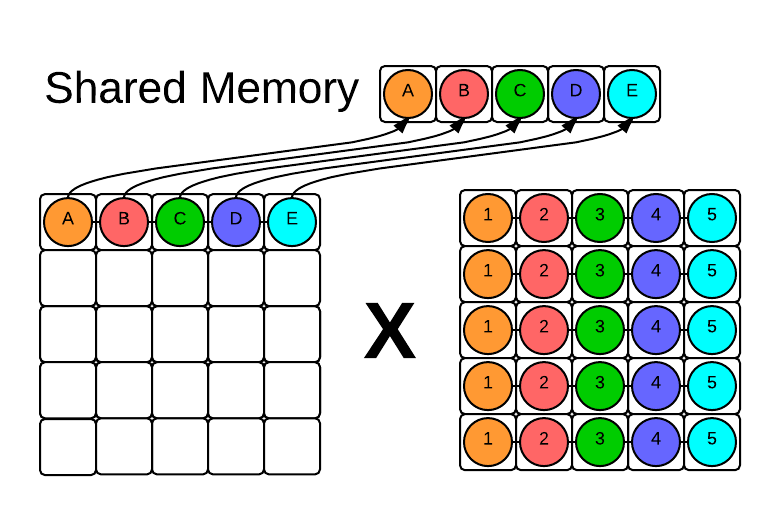
\includegraphics[width=3in]{ContractFieldFieldScalarGraphic}
    \caption[Memory accesses -- slicing]{Demonstration of memory accesses for the first team a slicing
        implementation of \texttt{ContractFieldFieldScalar}}
    \label{fig:Slicing}

    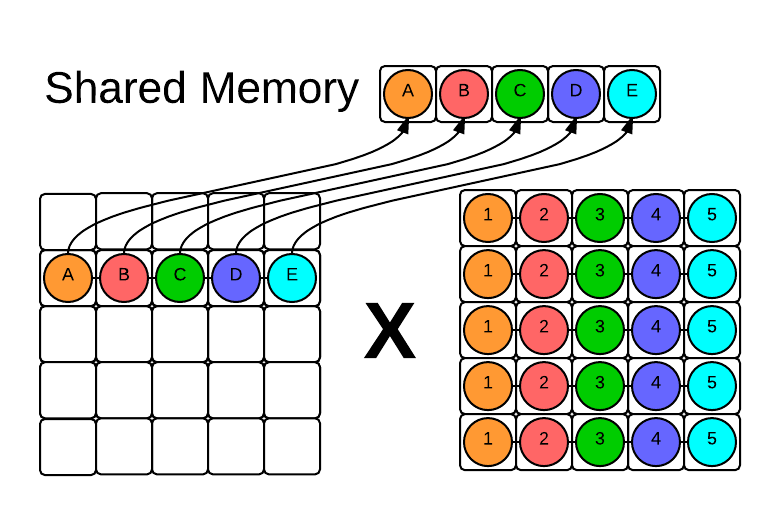
\includegraphics[width=3in]{ContractFieldFieldScalarGraphic2}
    \caption[Memory accesses -- slicing]{Demonstration of memory accesses for
    the second team of a slicing implementation of
    \texttt{ContractFieldFieldScalar}}
    \label{fig:Slicing2}
\end{figure}

We see that for the \texttt{ContractFieldFieldScalar} example, where our equation is given by
$A_{c,l,p} \times B_{c, r, p} = C_{c,l, r}$, the
number of teams initialized by the algorithm will be equal $l \times c$,
since there are $l$ teams per matrix, and we have $c$ matrices.
Additionally, there will be $r$ threads per team. 


    Kokkos code for executing the algorithm as described above is included in Figure~\ref{lst:ContractFieldFieldScalarSlice}. 

\begin{figure}[ht]
    \begin{lstlisting} [basicstyle=\tiny]
    int r = thread.team_rank();
    int c = thread.league_rank() / numLeftFields;
    int l = thread.league_rank() - c * numLeftFields; // (mod)

    // Load a slice into shared memory, each thread loads as many elements as it needs to.
    Kokkos::View<float*, Kokkos::MemoryUnmanaged> shared_slice(thread.team_shmem(), numPoints);
    for (int p = thread.team_rank(); p < numPoints; p += thread.team_size()) {
      shared_slice(p) = leftView(c, l, p);
    }
    thread.team_barrier();

    // Do as much as you can using that slice -- The parallel for goes across all the rows if possible.
    // This for loop is for the dot product within a row.
    float sum = 0;
    for (int p = 0; p < numPoints; ++p) {
      sum += shared_slice(p) * rightView(c, p, r);
    }
    outputView(c, l, r) = sum;

   \end{lstlisting}
\caption{Code from \texttt{ContractFieldFieldScalar} slicing
\label{lst:ContractFieldFieldScalarSlice}} 
\end{figure}

Another possible use of shared memory is to use tiles inspired by cache friendly
implementations of matrix multiplication. This approach will be discussed in
detail later, in Section~\ref{sec:tiling}, but it bears mentioning now for
contrast with the slicing approach.  The main advantage of slicing when compared
to a tile based approach is that it is easily generalizable to tensor
contractions of higher dimensions. Unlike tiling, which is significantly less
intuitive in higher dimensions, it is easy to implement slicing in higher
dimensions by loading a larger slice into shared memory.  Because of its
reliance on shared memory, we would expect it to perform poorly in situations
where the memory needed to store slices is a limiting factor. One class of
examples of this phenomenon are cases where the size of the contraction is large
relative to the number of basis functions. 

Intuitively, slicing is reliant on large contraction sizes to produce speedup
because in situations where the number of threads per team is low it is unable
to saturate the GPU. In flat parallelism, we use one thread per element in the
output matrix. Critically, these threads are not reliant one one another, so the
GPU does not have to satisfy constraints to give threads in the same team access
to shared memory. In contrast, slicing requires certain threads to be placed in
the same team, and when the size of a team is small (less than 100) this leads
to decreased performance.  This can be remedied by increasing the number of
contractions per team, but this risks introducing problems with shared memory.
Since shared memory is limited by nature (most NVIDIA GPUs offer only 48KB
shared memory), slicing has to balance the amount of work done per team with the
amount of shared memory available.
    
In situations where the contraction has an inherently large amount of reuse like
\texttt{ContractFieldFieldScalar}, this problem can be remedied to some degree
by loading multiple slices into shared memory and reusing them multiple times.
However, some contractions, like \texttt{ContractDataDataScalar}, do not reuse
any of the elements in the left input matrix to calculate multiple output
elements. In these cases, it seems clear that slicing will not be an efficient
algorithm. 
	
When we compare slicing approaches using one contraction per team to independent
flat parallelism on \texttt{ContractFieldFieldScalar}, we get underwhelming
results, as shown by Figure~\ref{fig:CFFSSlicingVSIndepentent}. 

\begin{figure}[!ht] 
    \centering
    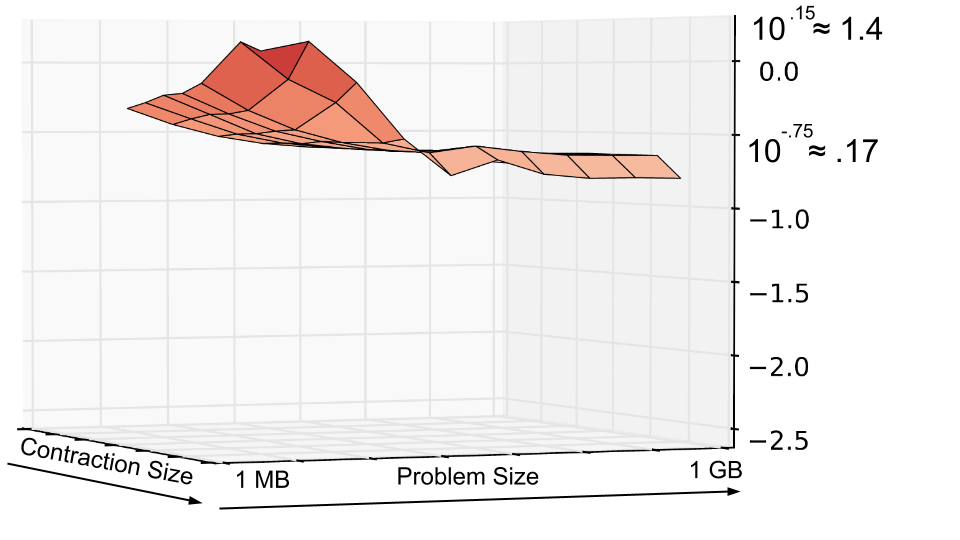
\includegraphics[width=5in]{CFFS_Slicing}
    \caption[\texttt{ContractFieldFieldScalar} speedup over
    flat parallel]{\texttt{ContractFieldFieldScalar} slicing speedup compared to
    flat (interactionless) parallelism}
\label{fig:CFFSSlicingVSIndepentent}
\end{figure}


These results were generated by comparing independent algorithms to slicing on
\texttt{ContractFieldFieldScalar} with $l = r = 10$ and $p \in [8,1024]$. We see
that in the corner where the memory size is small and contraction size is small
we get a small amount of speedup relative to flat Cuda code, which is
promising. This is the corner where we would expect slicing to perform the best
with respect to independent parallelism, since in this corner flat parallelism
is unable to fully saturate the GPU. The benefits of reuse in this corner are
significant enough to out-compete flat parallelism. On the rest of the graph,
however, the inability of slicing to saturate the GPU means that it is
significantly slower that flat parallelism. Since $l = r = 10$,
the algorithm naturally only spawns 10 threads per team, which, as previously discussed, is not enough. 

Fortunately, this can be counteracted to some degree by loading multiple slices 
into shared memory simultaneously. This places a larger strain on shared memory, 
but also presents additional opportunities for parallelism. 
This technique has shown promising results on \texttt{ContractFieldFieldTensor}, as shown in Figure~\ref{fig:TwoSlicings}. 

\begin{figure}[H]
    \centering
    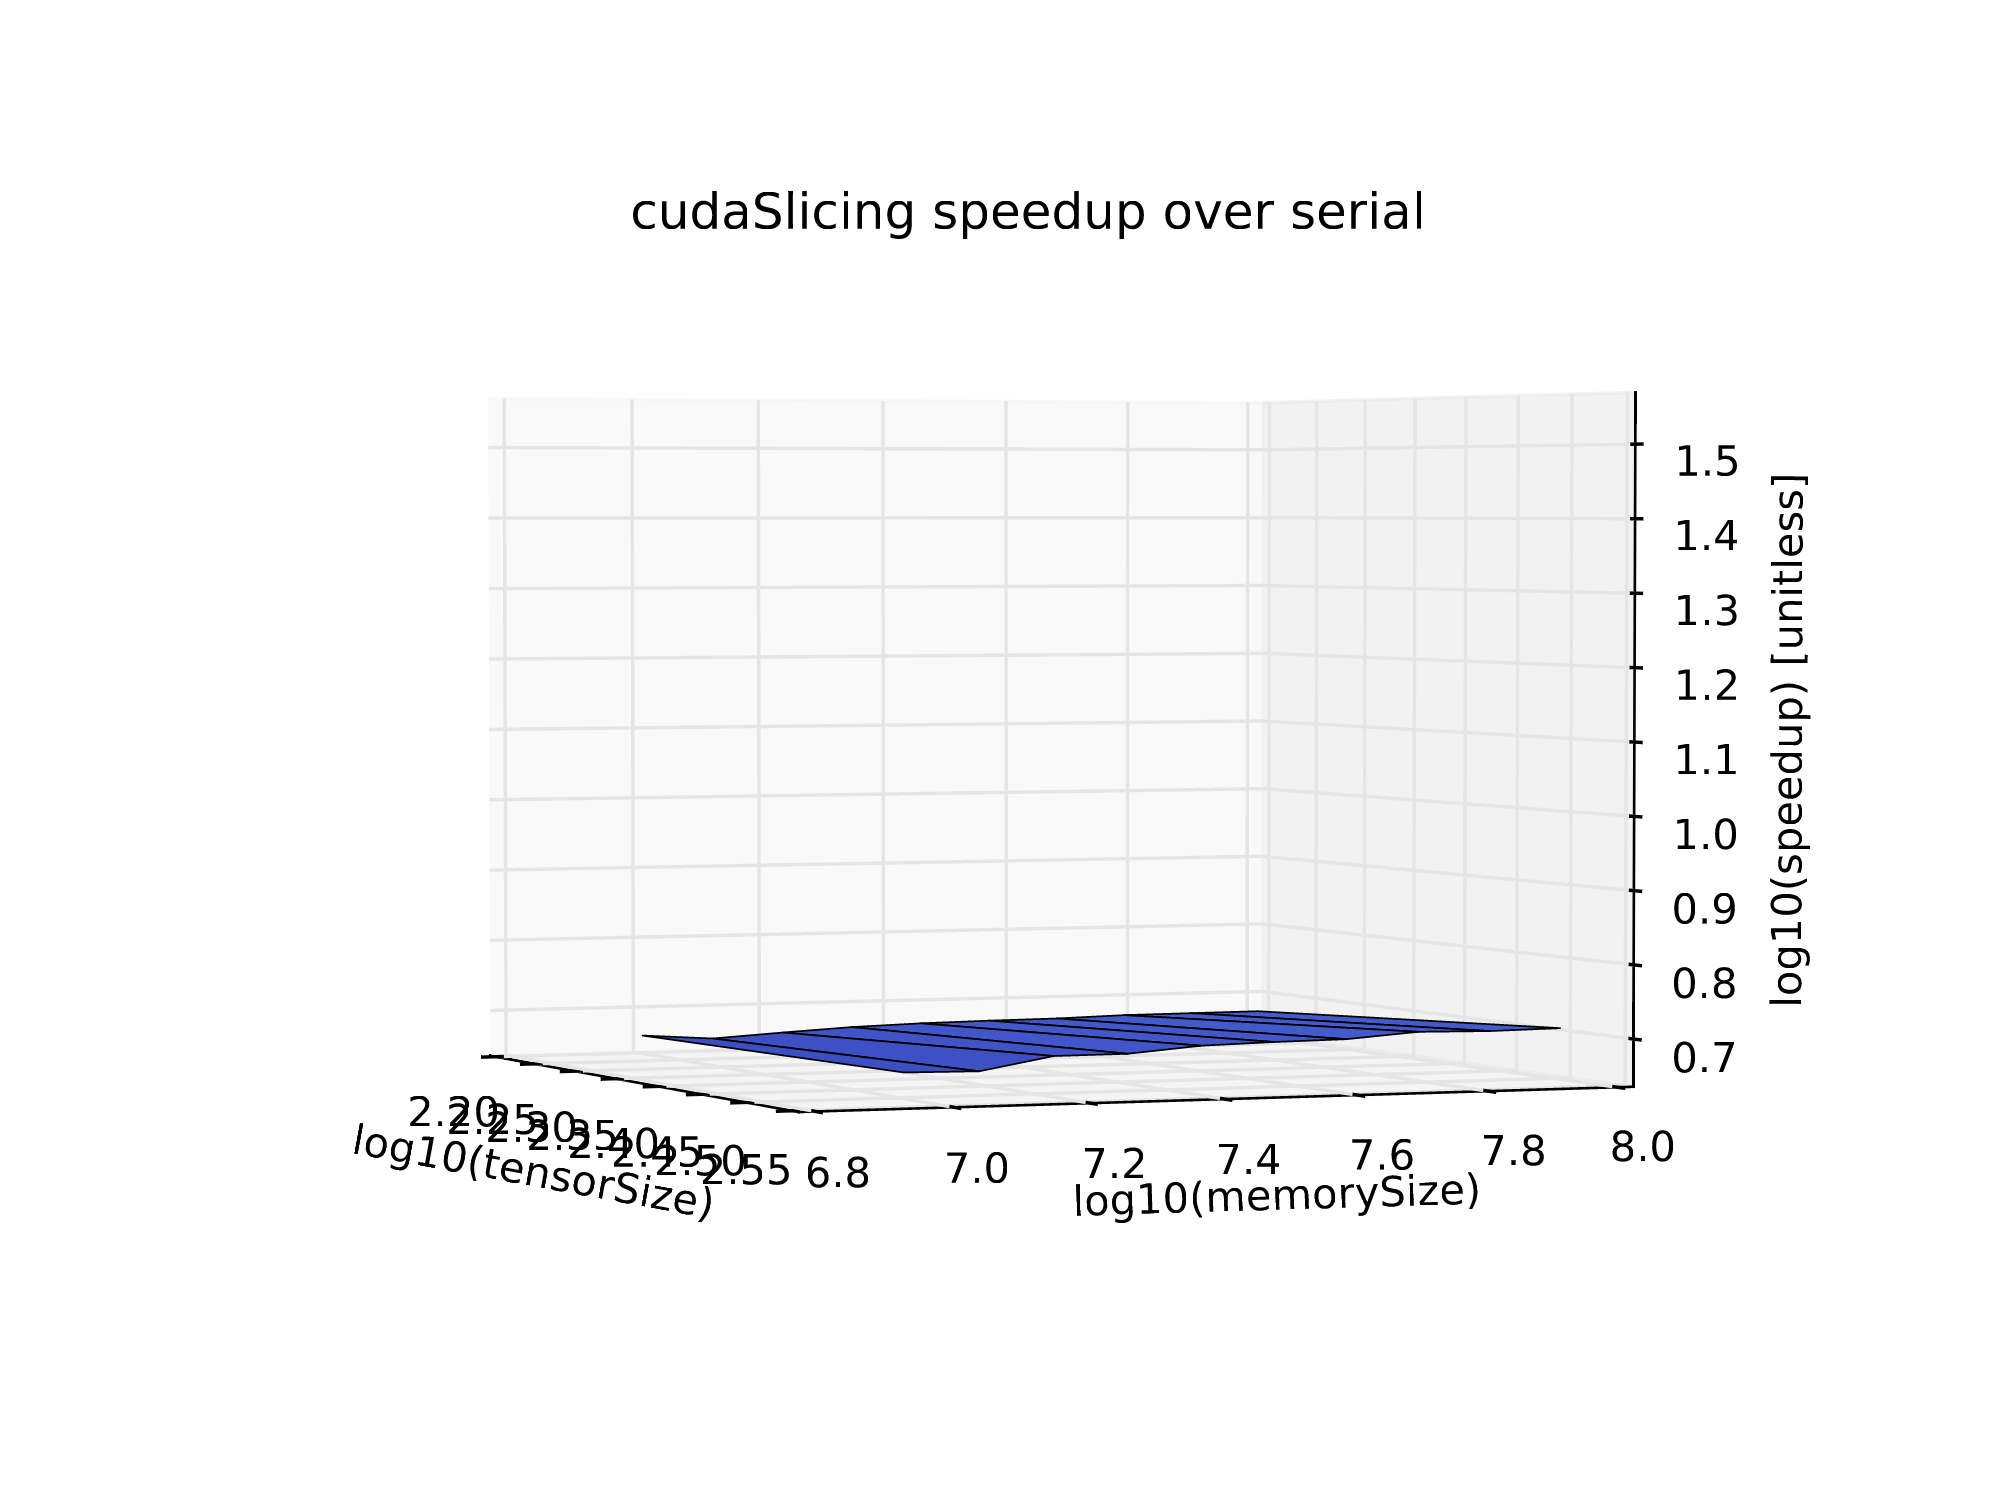
\includegraphics[width=5in]{CFFTSlicingVSSerial}
    \caption{Performance of slicing parallelism when compared to serial}

    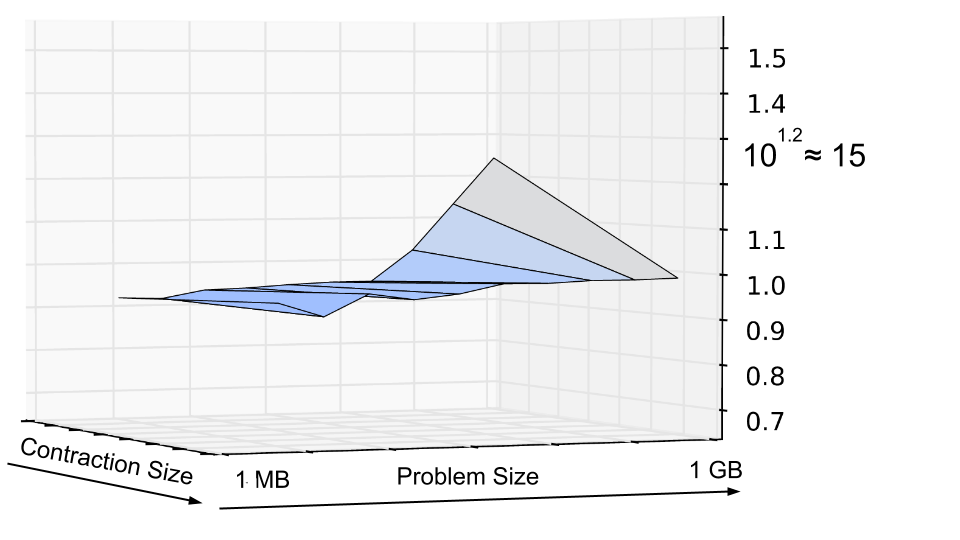
\includegraphics[width=5in]{CFFTAdaptiveSlicingVSSerial}
    \caption[Performance of adaptive slicing]{Performance of Adaptive Slicing on
    the same problem, note the increased speedup}
\label{fig:TwoSlicings}
\end{figure}

This shows that the adaptive slicing approach does have some promise in these applications. These results were generated by loading two slices simultaneously in \texttt{ContractFieldFieldTensor} with $l = r = 125$, $d_1 = d_2 = 4$, and $p$ ranging from $160$ to $320$.

% Alex
\section{Tiling}\label{sec:tiling}

The final parallelization technique we used for these tensor contractions was
tiling. This technique is similar to the tiled technique for matrix
multiplication used in serial operations. Instead of relying on the cache to
retain the relevant pieces of information, however, we use shared memory to
explicitly store the data we care about. Once again, we will explain this
algorithm by example. Consider one of the matrix multiplications in
\texttt{ContractFieldFieldScalar} as shown in Figure~\ref{fig:Tiling}. 


\begin{figure}[!ht]
    \centering
    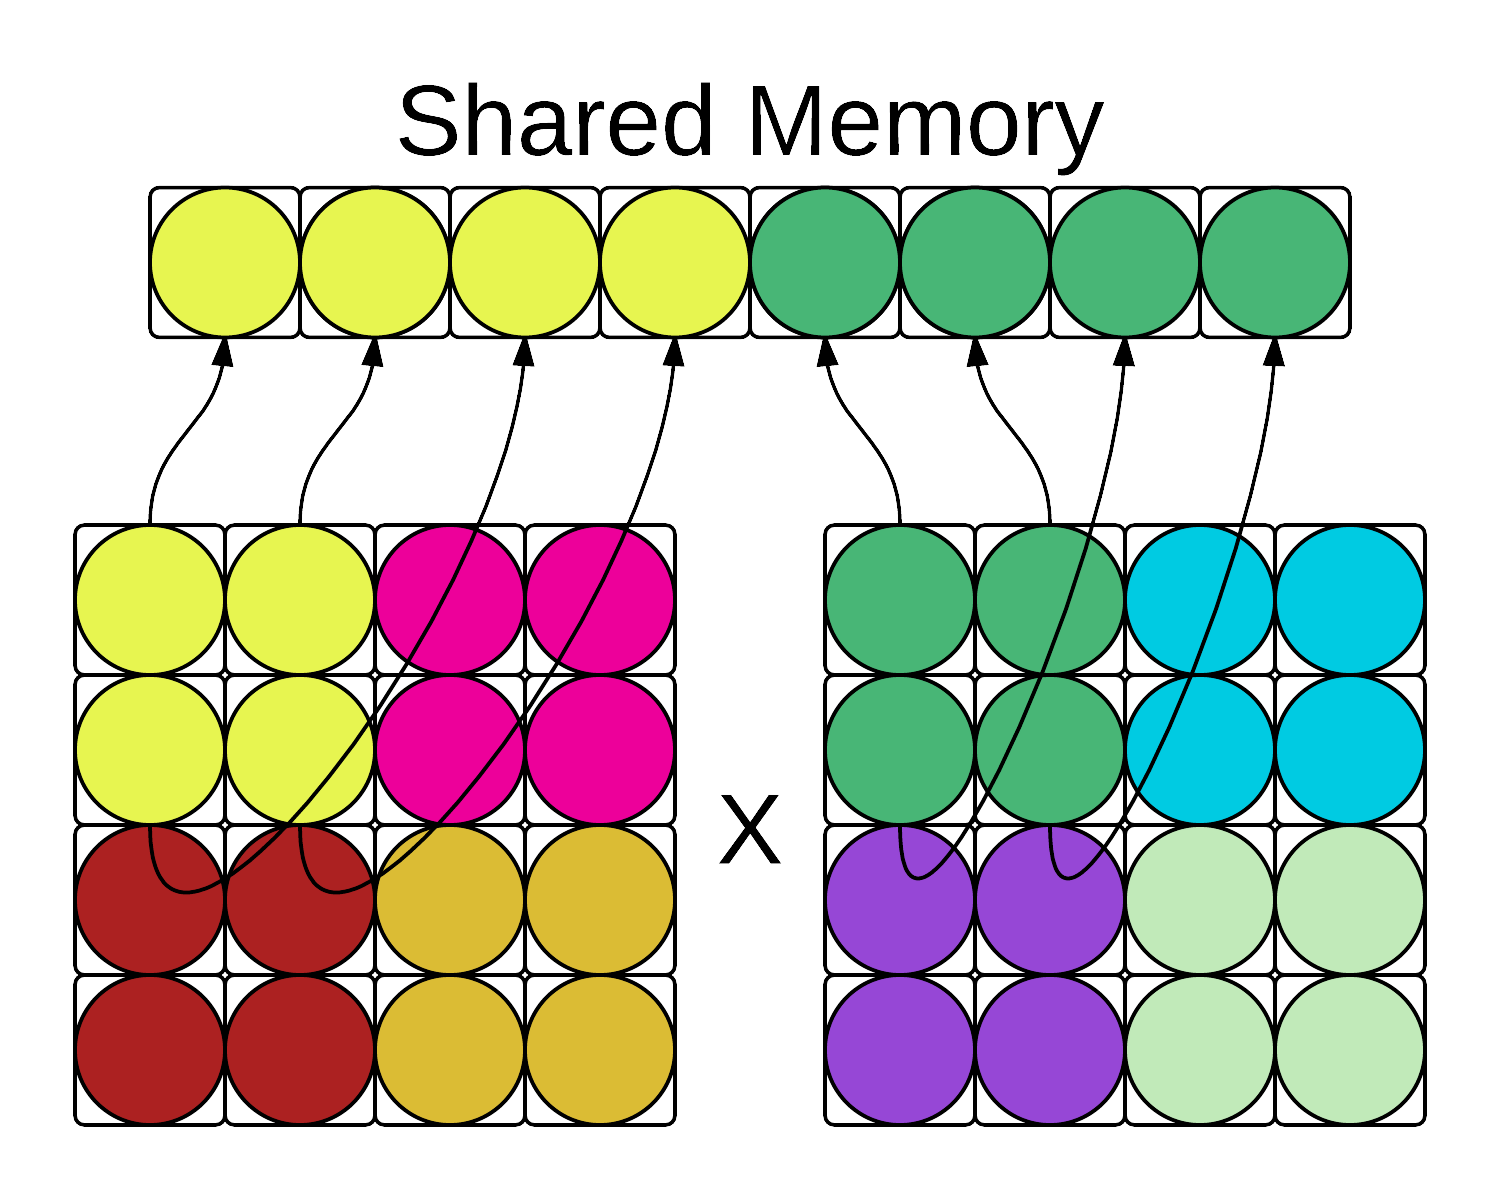
\includegraphics[width=2in]{SharedMem1.png}
    \caption[Memory accesses -- tiling]{Demonstration of first round of memory
        accesses for a tiling implementation of \texttt{ContractFieldFieldScalar}}
    
    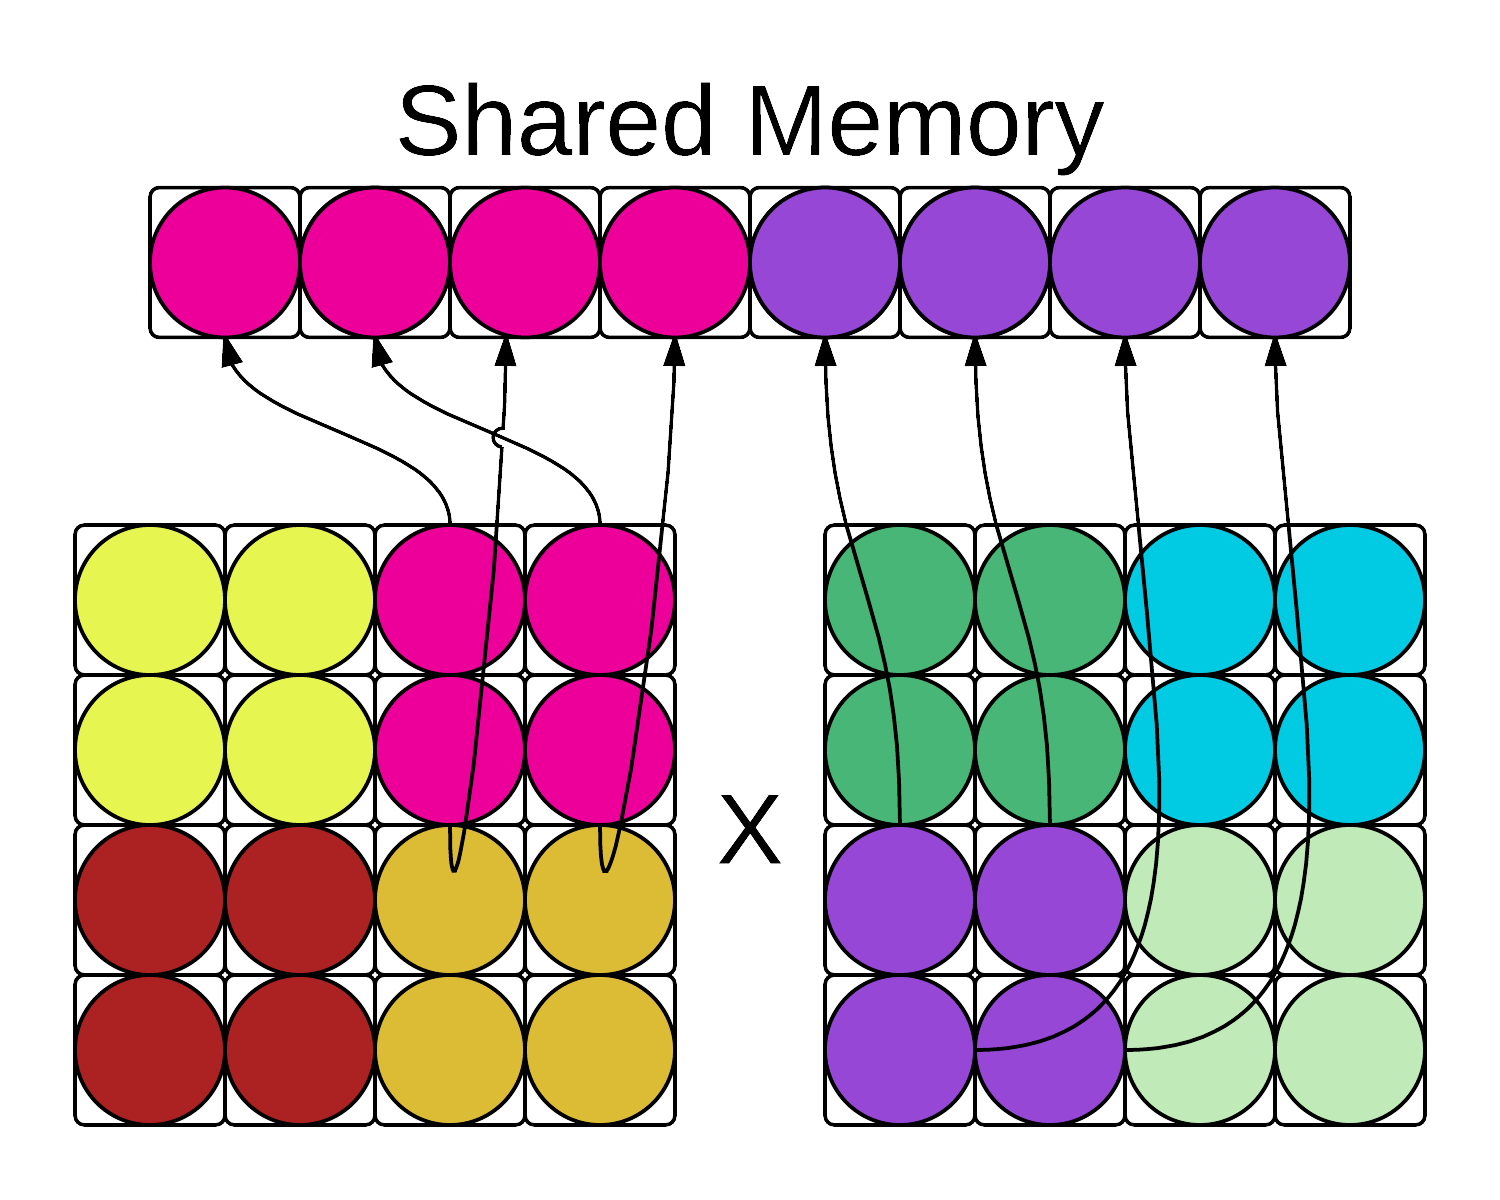
\includegraphics[width=2in]{SharedMem2.png} \caption[Memory accesses --
    tiling]{Demonstration of second round of memory accesses for a tiling
        implementation of \texttt{ContractFieldFieldScalar}}
\label{fig:Tiling}
\end{figure}

For the sake of simplicity we'll consider a team to be four threads, which
simplifies our computation since the matrix is four by four. On the left hand
side, the team loads a four element tile into the shared memory of the
threads. Once these elements are loaded into memory, each thread can begin
computation of their element in the output matrix. Each thread computes as much
of their output element as they can using the elements in shared memory, then
we load a new tile into shared memory and continue the process, as shown in Figure~\ref{fig:Tiling}.
We see that in this case we will have to load two tiles into shared memory
before we have computed every output element in the first tile in its entirety. 


    Tiling can be viewed as a more specialized version of slicing, since they
both use similar access patterns for shared memory. The difference between the
two lies in tiling's usage of multiple contractions per team, as well as the
the distribution of a contractions operations over multiple loops of the
routine. Because of these differences, tiling can routinely saturate the GPU in
a way that pure slicing cannot, since the algorithm inherently limits the
shared memory usage per team by reusing the same shared memory multiple times.
Additionally, if we set the dimension of our tiles such that the width of a tile
squared is the appropriate number of threads per team for GPU performance, the algorithm
saturates the GPU with both teams and threads. This is much more difficult to do 
adaptively using pure slicing. 
	
    Excerpts from our Kokkos implementation of tiling are included in Figure~\ref{lst:ContractFieldFieldScalarTilingCode}. The
code assumes that \texttt{tileSize} (the horizontal and vertical dimensions of a tile)
evenly divides both the contraction size and $l = r =
\text{numBasis}$.
	
\begin{figure}[H]
    \begin{lstlisting} [basicstyle=\tiny]
    
    const unsigned int numBasis = numLeftFields;

    // We use -1, +1 to get the ceiling of numPoints/tile_size and numBasis/tile_size
    const unsigned int numberOfPointTiles = numPoints / tile_size;
    const unsigned int numberOfBasisTiles = numBasis / tile_size;

    const unsigned int numberOfTiles = numCells * numberOfBasisTiles * numberOfBasisTiles;

    const unsigned int subRow = thread.team_rank() / tile_size;
    const unsigned int subCol = thread.team_rank()  - subRow * tile_size; // (mod)

    // Create our tiles
    Kokkos::View<float**, Kokkos::MemoryUnmanaged> LeftTileStorage(thread.team_shmem(), tile_size, tile_size);
    Kokkos::View<float**, Kokkos::MemoryUnmanaged> RightTileStorage(thread.team_shmem(), tile_size, tile_size);

    const unsigned int resultMatrix = resultTileIndex / (numberOfBasisTiles * numberOfBasisTiles);
    const unsigned int resultSubmatrixIndex = resultTileIndex - (resultMatrix * numberOfBasisTiles * numberOfBasisTiles); // (mod)

    // calculate result tile indices
    const unsigned int resultTileRow = resultSubmatrixIndex / numberOfBasisTiles;
    const unsigned int resultTileCol = resultSubmatrixIndex  - resultTileRow * numberOfBasisTiles;

    // calculate this threads actual output index
    const unsigned int row = resultTileRow * tile_size + subRow;
    const unsigned int col = resultTileCol * tile_size + subCol;

    float sum = 0;
    // for tileNumber in 0...numberOfTilesPerSide
    for (unsigned int tileNumber = 0;
        tileNumber < numberOfPointTiles; ++tileNumber) {

      // load the left and right tiles into shared memory
      LeftTileStorage(subRow, subCol)  = leftView(resultMatrix, row, tileNumber * tile_size + subCol);
      RightTileStorage(subRow, subCol) = rightView(resultMatrix, tileNumber * tile_size + subRow, col);
      
      // make sure everyone's finished loading their pieces of the tiles
      thread.team_barrier();
      for (unsigned int dummy = 0; dummy < tile_size; ++dummy) {
        sum += LeftTileStorage(subRow, dummy) *
            RightTileStorage(dummy,subCol);
        }
        thread.team_barrier();
   }
   outputView(resultMatrix, row, col) = sum;
 \end{lstlisting}
 \caption[\texttt{ContractFieldFieldScalar} tiling implementation]{A
     Kokkos implementation
     of the \texttt{ContractFieldFieldScalar} functor using tiling. Note the change 
     in data shape as described in \ref{sec:Slicing}}
 \label{lst:ContractFieldFieldScalarTilingCode}
\end{figure}


Thus far in our research, we have found tiling to be the most effective
algorithm for realizing parallel speedup. 

\begin{figure}[H]
    \centering
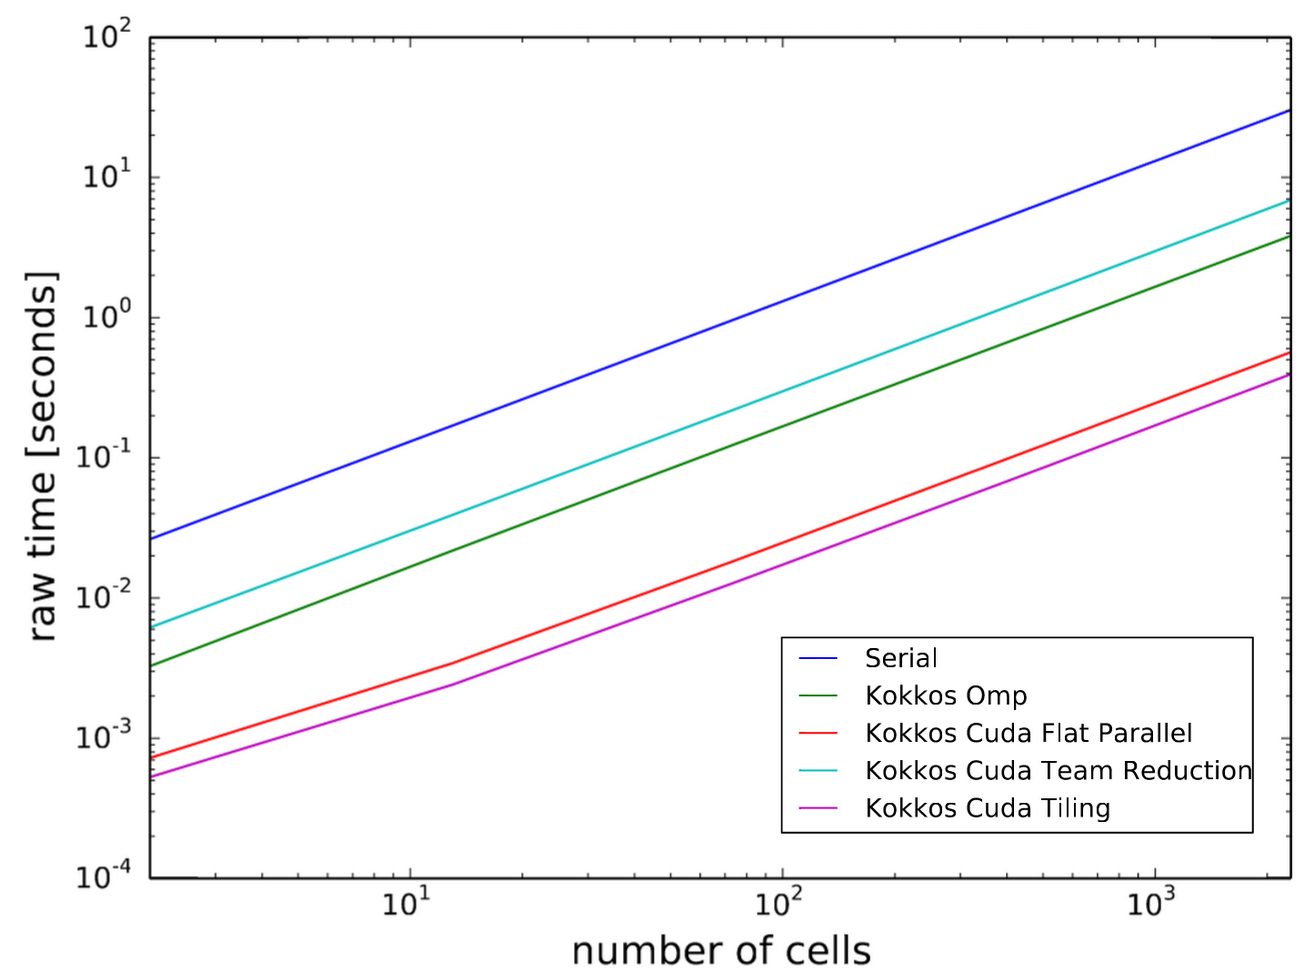
\includegraphics[width=5in]{CFFS_RawTimes_LR125P216_2.PNG} 
\caption[\texttt{ContractFieldFieldScalar} performance summary (large)]{Raw times
    for many different algorithms used for \texttt{ContractFieldFieldScalar}.
    Note that Tiling is the best performing (lowest). This data was generated
    with
    $l=r=125$, $p=216$}
\label{fig:TilingPerformance}
\end{figure}
Consider the graph generated in Figure~\ref{fig:TilingPerformance} for \texttt{ContractFieldFieldScalar}. We see that tiling outperforms both flat parallelism and team reductions across the board. This trend continues for smaller use cases as well, as shown in Figure~\ref{fig:TilingPerformance2} when $l = r = 8$, $p = 8$.

\begin{figure}[H]
    \centering
    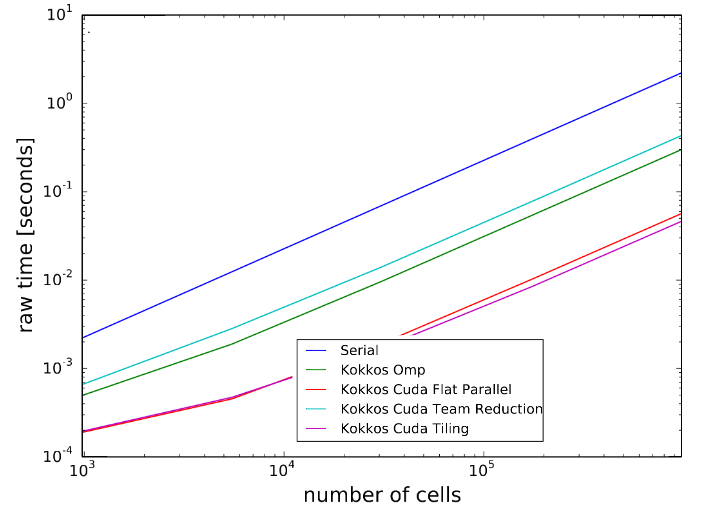
\includegraphics[width=5in]{CFFS_RawTimes_LRP8_2.PNG}
    \caption[\texttt{ContractFieldFieldScalar} performance summary (small)]{Raw
        times for many different algorithms used for \texttt{ContractFieldFieldScalar}.
        This data was generated with $l=r=8$, $p=8$}
\label{fig:TilingPerformance2}
\end{figure}

\subsection{ContractFieldFieldTensor}

We also created a tiling implementation of \texttt{ContractFieldFieldTensor}. Conceptually, it is much more difficult to envision how to approach tiling on multidimensional problems. \texttt{ContractFieldFieldTensor}, which can be described by the equation $A_{c,l,p,d_1,d_2} \times B_{c, r, p,d_1,d_2} = C_{c,l, r}$, therefore presents an interesting problem for the tiling approach. 

Unlike slicing, there seem to be multiple distinct ways of approaching the
problem. One can unroll the entire contraction to create a situation where
the left and right matrices are rectangular, but can be covered by 2D tiles.
Alternatively, algorithms could cover the left and right inputs using
multidimentional tiles. While conceptually these two approaches seem distinct,
they are functionally equivalent. Ultimately, tiling involves loading pieces of
both the input and output matrices into shared memory and operating on them
repeatedly. As long as we avoid suboptimal memory access patterns, it makes no
difference whether we visualize the tiles as two dimensional or with even higher
dimensions. For ease of understanding, we implemented
\texttt{ContractFieldFieldTensor}'s tiling kernels with unrolled
contractions. This essentially, reduces the kernel to a series of long dot
products in our vision of the memory layout. 

Using the tiling method on \texttt{ContractFieldFieldTensor} we were able to generate speedup of between $1.5$ and $1.7$ times over flat parallelism, as shown in Figure~\ref{fig:CFFTSpeedup}. 

\begin{figure}[H]
    \centering
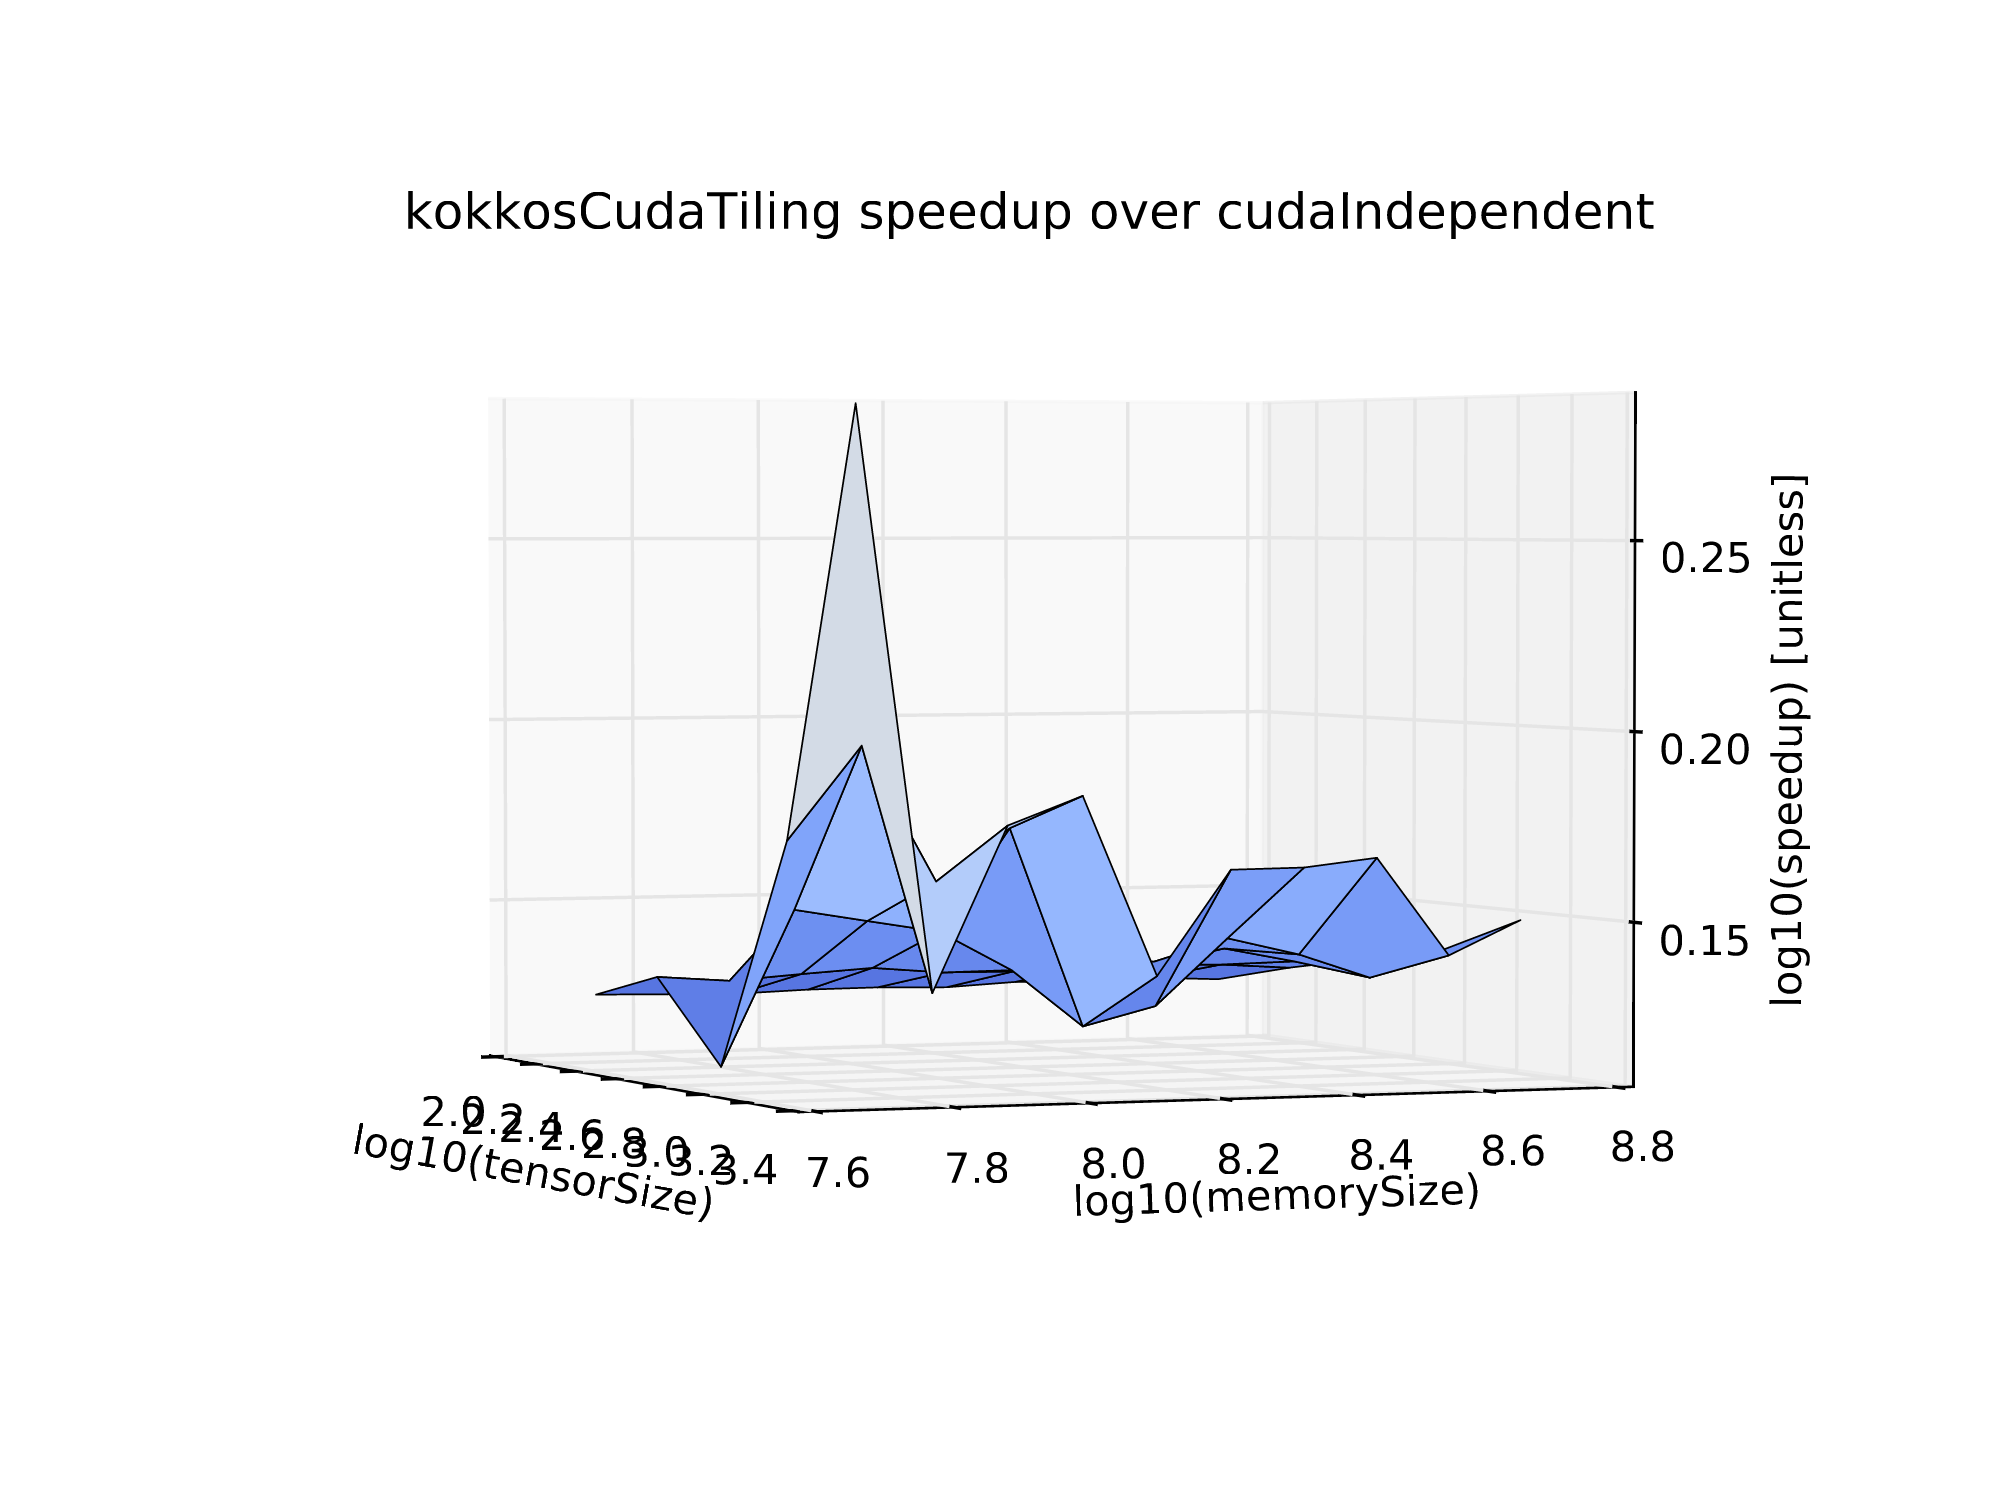
\includegraphics[width=5in]{ContractFieldFieldTensor}
\caption[\texttt{ContractFieldFieldScalar} Tiling performance]{Speedup of Tiling
    for \texttt{ContractFieldFieldTensor} over independent parallelism. This data was
    generated with $l = r = 16$, $d_1 =
d_2 = 4$, and $p$ varying from 16 to 128. The tile size used was 16.}
\label{fig:CFFTSpeedup}
\end{figure}

In this case, the number of GPU teams
capable of working on a contraction using the tiling algorithm is given by
$\frac{\text{number of basis functions}}{\text{size of a tile}}$, where the number of basis functions
is the number of contractions per left and right matrix. As long as this number
is sufficiently high, as it was in all of the use cases we were concerned with, 
tiling should theoretically perform well in these use cases, as shown by
Figures~\ref{fig:multiDTiling1} and \ref{fig:multiDTiling2}.

\begin{figure}[H]
    \centering
    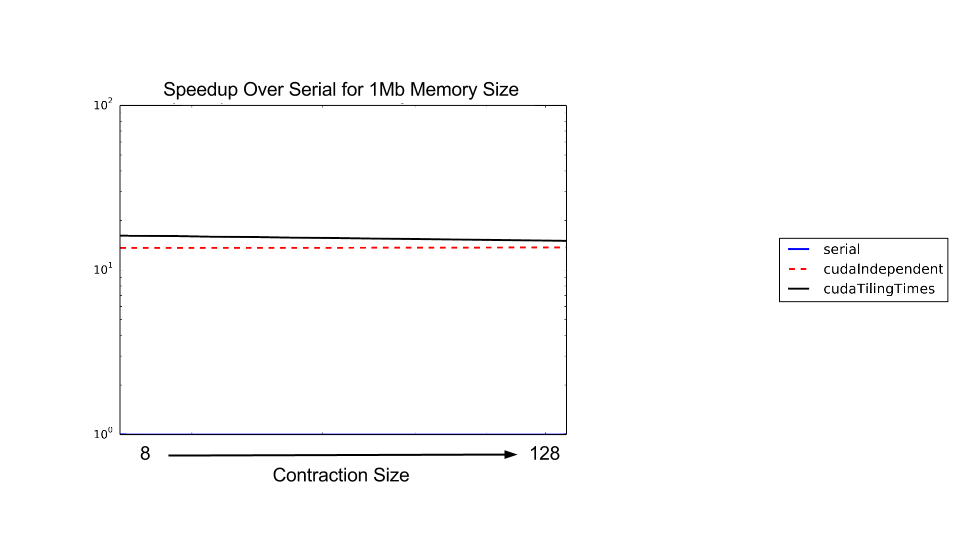
\includegraphics[width=5in]{CFFTTiling1}
    \caption[\texttt{ContractFieldFieldScalar} tiling (small
    memory)]{Speedup for serial, independent, and tiling approaches to
        \texttt{ContractFieldFieldScalar}.  This data was generated with
        $l=r=16$, $d_1=d_2=4$, with $p$
varying from $8$ to $128$. This graph uses a relatively low memory size, which
limits the number of cells}
\label{fig:multiDTiling1}
\end{figure}

\begin{figure}[H]
    \centering
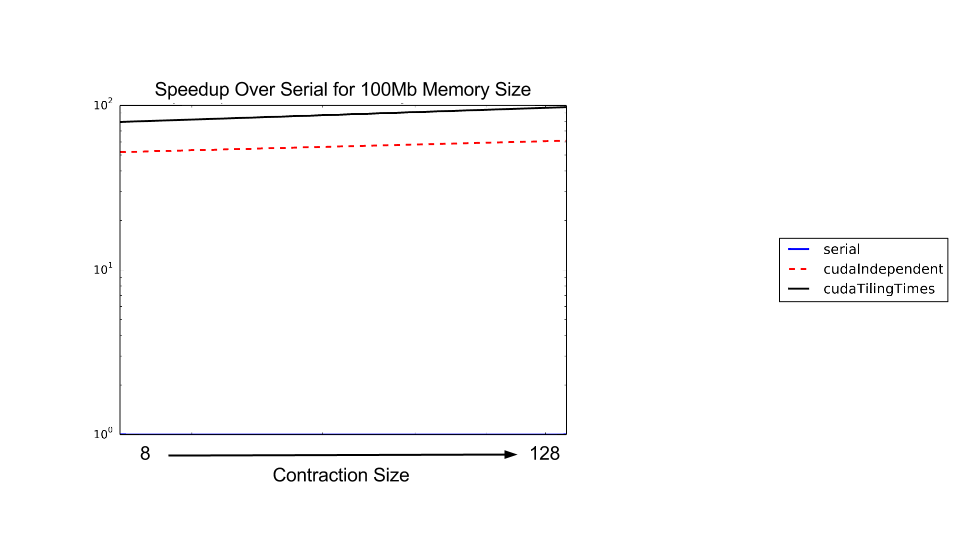
\includegraphics[width=5in]{CFFTTiling2}
\caption[\texttt{ContractFieldFieldScalar} tiling (large
memory)]{Speedup for serial, independent, and tiling approaches to
    \texttt{ContractFieldFieldScalar}. This data was generated with
    $l=r=16$, $d_1=d_2=4$, with $p$ varying from $8$ to $128$. This
data was collected while simulating a memory size an order of magnitude larger
than the previous image, leading to a significantly higher cell count. }
\label{fig:multiDTiling2}
\end{figure}

Excerpts from our implementation of tiling for \texttt{ContractFieldFieldTensor} are included in Figure~\ref{lst:CFFTTilingCode}, which have been simplified using the assumption that $l=r$ as well as the assumption that the size of each tile evenly divides every other dimension for clarity. 

\begin{figure}[H]
    \begin{lstlisting} [basicstyle=\tiny]

    // Here we pretend that all three contraction dimensions are a single dimension: contractionSize
    const unsigned int contractionSize = _dimTens1 * _dimTens2 * _numPoints;
    
    const unsigned int numberOfPointTiles = contractionSize / tile_size;
    const unsigned int numberOfBasisTiles = numBasis / tile_size;

    const unsigned int numberOfTiles = _numCells * numberOfBasisTiles * numberOfBasisTiles;
    
    //These are the subRow and subColumn of the thread within its tile
    const unsigned int subRow = thread.team_rank() / _tile_size;
    const unsigned int subCol = thread.team_rank() - subRow * _tile_size;

    unsigned int resultTileIndex = thread.league_rank();
    //Our shared memory for the computation, which fits two full tiles
    Kokkos::View<float*, Kokkos::MemoryUnmanaged> tileStorage(thread.team_shmem(), 2 * _tile_size * _tile_size);

    const unsigned int resultMatrix = resultTileIndex / (numberOfBasisTiles * numberOfBasisTiles);
    const unsigned int resultSubmatrixIndex = resultTileIndex - (resultMatrix * numberOfBasisTiles * numberOfBasisTiles); // (mod)

    // calculate result tile indices
    const unsigned int resultTileRow = resultSubmatrixIndex / numberOfBasisTiles;
    const unsigned int resultTileCol = resultSubmatrixIndex - resultTileRow * numberOfBasisTiles; // (mod)

    // calculate this threads actual output index
    const unsigned int row = resultTileRow * _tile_size + subRow;
    const unsigned int col = resultTileCol * _tile_size + subCol;
    float sum = 0;

    // for tileNumber in 0...numberOfTilesPerSide
    for (unsigned int tileNumber = 0; tileNumber < numberOfPointTiles; ++tileNumber) {

        // these are base indices into the shared memory
        const unsigned int leftBaseIndex = subRow * _tile_size;
        const unsigned int rightBaseIndex = _tile_size*_tile_size + subCol;

        // Here we break it back down so that we can use it
        const unsigned int leftContractionIndex = tileNumber*_tile_size + subCol;
        const unsigned int left_qp = leftContractionIndex / (_dimTens1*_dimTens2);
        const unsigned int left_combinedTens = leftContractionIndex - left_qp * (_dimTens1 * _dimTens2); // (mod)
        const unsigned int left_iTens1 = left_combinedTens / _dimTens2;
        const unsigned int left_iTens2 = left_combinedTens - left_iTens1 * _dimTens2; // (mod)

        const unsigned int rightContractionIndex = tileNumber * _tile_size + subRow; 
        const unsigned int right_qp = rightContractionIndex / (_dimTens1*_dimTens2);
        const unsigned int right_combinedTens = rightContractionIndex - right_qp * (_dimTens1 * _dimTens2); // (mod)
        const unsigned int right_iTens1 = right_combinedTens / _dimTens2;
        const unsigned int right_iTens2 = right_combinedTens - right_iTens1 * _dimTens2; // (mod)

        // load the left and right tiles into shared memory
        tileStorage(thread.team_rank()) = _leftView(resultMatrix, row, left_qp, left_iTens1, left_iTens2);
        tileStorage(thread.team_rank() + (_tile_size * _tile_size)) =
            _rightView(resultMatrix, right_qp, right_iTens1, right_iTens2, col);

        // make sure everyone's finished loading their pieces of the tiles
        thread.team_barrier();

        for (unsigned int dummy = 0; dummy < _tile_size; ++dummy) {
          sum +=
            tileStorage(leftBaseIndex + dummy) *
            tileStorage(rightBaseIndex + dummy * _tile_size);
        }
        thread.team_barrier();
      }
      
      _outputView(resultMatrix, row, col) = sum;
      
 \end{lstlisting}
 \caption[Tiling implementation code]{Code for Kokkos implementation of tiling
     for \texttt{ContractFieldFieldTensor}}
\label{lst:CFFTTilingCode}
\end{figure}
 
 
           % brett, ellen, alex
    % Flat parallelism (Brett)
    % Reduction (Ellen)
    % Slicing (Alex)
    % Tiling (Alex)

% Brett
\chapter{Experience with Kokkos}
\section{Performance}
%Comparing Kokkos to Cuda and OpenMP
%Doing this for sanity check
%How we did this (used same algorithm and ran both, timed)
%some graphical results
%analysis of the results and differences
%conclusion that they are very similar performing
A feature that many programmers consider when deciding what the best solution is
to solve their problem, is performance. Since Kokkos uses Cuda and OpenMP as a
backend we thought that it was important to do some testing to ensure that
Kokkos performs as well as these two solutions. If Kokkos's performance was
worse then Cuda's or OpenMP's then programmers would use these other solutions
instead. The good news for Kokkos is that in our testing it performs almost
identically to Cuda and OpenMP. We did not spend an extensive amount of time
confirming our results due to project priorities, but after a few pieces of supporting data we assumed that
the rest of the tests would give similar results because there is no information or evidence
that should give us reason to believe this trend will change. The rest of this
section will describe our strategy for testing performance of Kokkos versus Cuda
and Kokkos versus OpenMP, present graphs showing the differences observed, and
analyze the graphs.

The general method that was used to create performance data for Kokkos, Cuda,
and OpenMP was to write algorithmically equivalent code for all three, make sure
that the layout of the data is the same, then time the runtime of each (one
after another). This process is pretty simple, but there is always noise in
timing. That is why we repeated the same exact calculation five times and 
then use the average time. A couple things that should be noted are we are
unsure how Kokkos does a reduction in the team\_reduce() function, meaning we
could not write a Cuda reduction that we knew was algorithm equivalent, and we
can not be sure that the compilers do the same optimizations. Although
we could have asked Dr. Carter Edwards (our liaison and one of the creators of 
Kokkos), the project's priorities had changed and it was decided to not pursue
this further. Regarding the second note, we tried to manually do some code
optimizations that compilers can handle in order to make sure the amount of work
each algorithm was the same (which is expected). Of course if one compiler has
more advanced optimization techniques that is a benefit that should not be
overlooked, but the goal of this testing was not to test performance against
ease of coding, but rather the overall performance differences of Kokkos to 
Cuda and Kokkos to OpenMP. 

Now we will look at some of the performance differences and similarities of
Kokkos, Cuda, and OpenMP. Here is a graph that shows the raw times of Kokkos
Cuda, Cuda, Kokkos OpenMP, and OpenMP for ContractDataDataScalar: \\
\begin{figure}[!ht]
{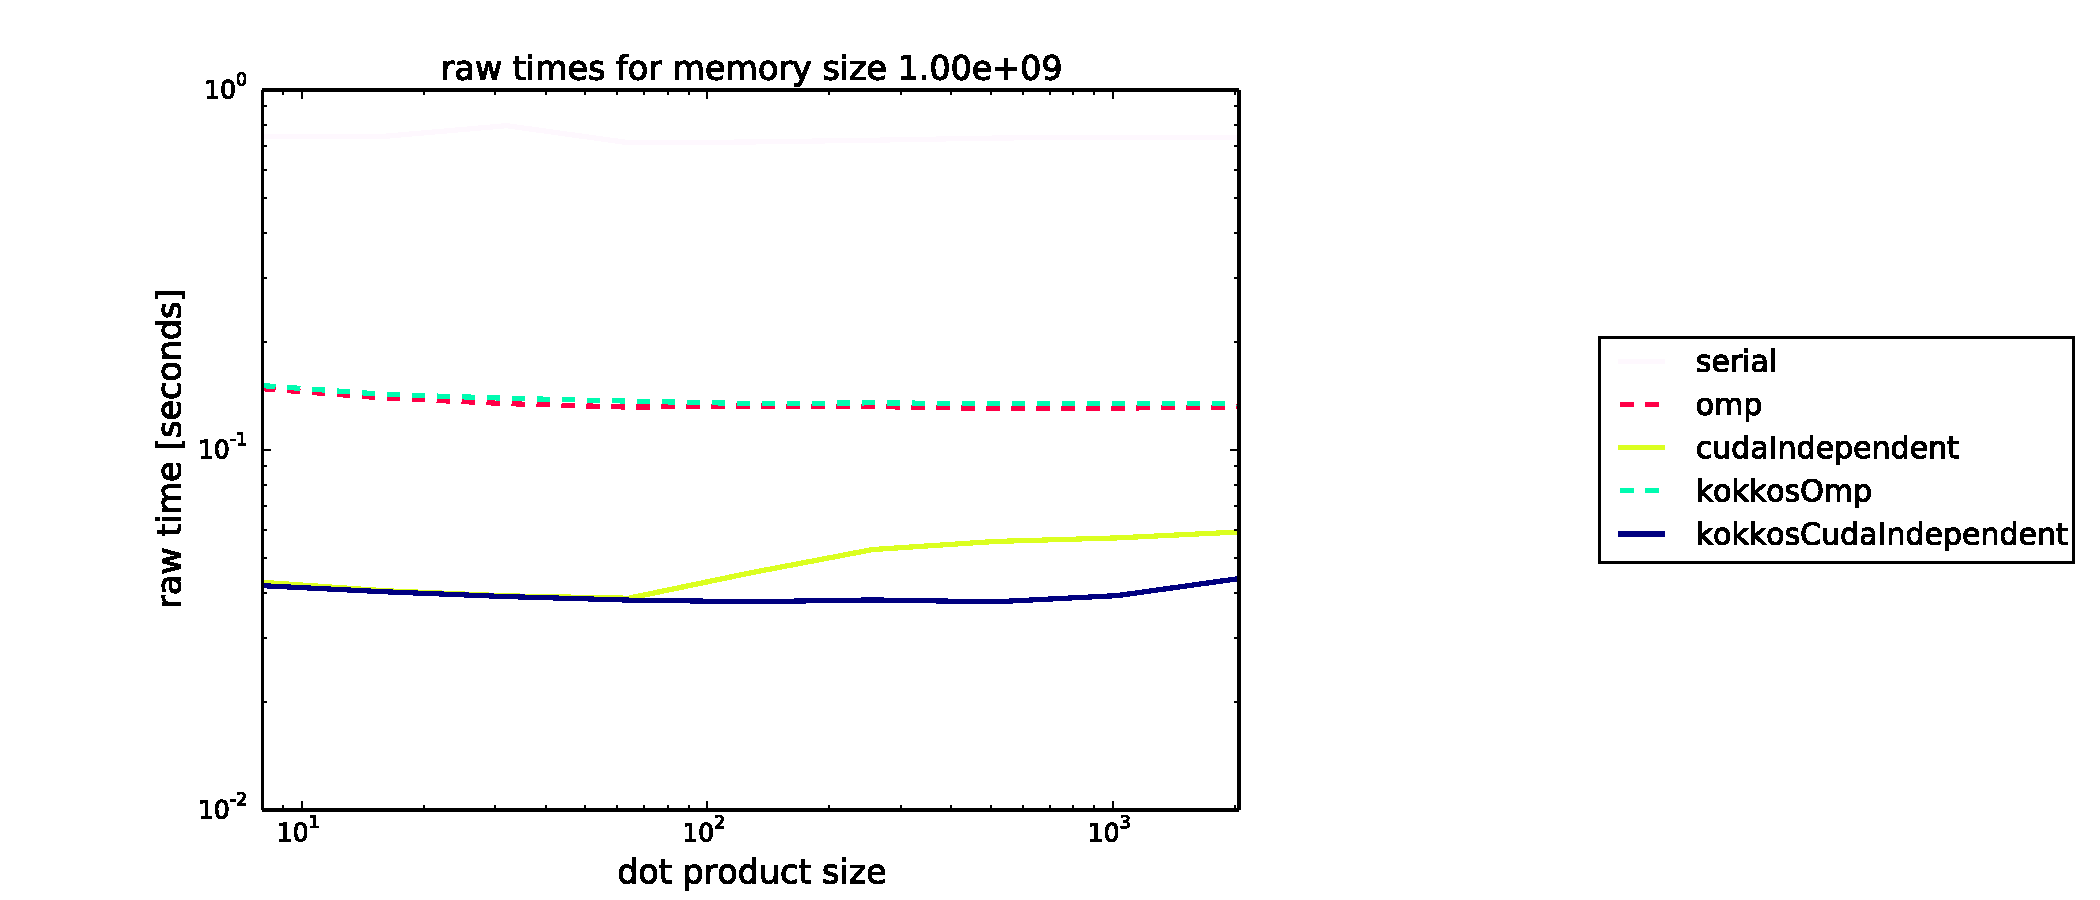
\includegraphics[scale=.4]{CDDS_RawTimes_2d_largestSize_Comparison.pdf}}
\caption[ContractDataDataScalar Kokkos performance comparison]{This graph plots the performance of Kokkos Cuda, Cuda, Kokkos OpenMP,
and OpenMP for ContractDataDataScalar with a memory size of 1 GB. 
The y-axis is time in
seconds, so closer to 0 is better. The x-axis plots different contraction sizes
in order to compare multiple points.}
\label{fig:ContractDataDataScalar Kokkos performance comparison}
\end{figure} \\
Notice how in this graph Kokkos OpenMP and OpenMP are almost perfectly
overlapping with Kokkos OpenMP. We are not quite sure why they are not perfectly
overlapping, but it appears that it is not random noise because it is pretty
consistent in this graph. However, the difference is so small it seems
insignificant. 

KokkosCuda versus Cuda, on the other hand, has some big differences. They are
identical for the smaller problems but diverge a significant amount for bigger
problems. This trend exists because Kokkos is launching a different amount of blocks than the number of blocks Cuda launches 
(Kokkos launches fewer blocks, with the intention of reusing them).
We believe the reason this doesn't effect the smaller problem sizes is because
the number of blocks that needs to be launched is smaller than the bigger problem sizes, so
the upper limit of number of blocks launched is not reached, but clearly is in the bigger problem sizes. 

Now here is a graph for ContractFieldFieldScalar that includes the slicing technique (which uses shared memory)
for both Kokkos Cuda and Cuda and it includes the normal flat parallel algorithm for Kokkos Cuda and Cuda. \\
\begin{figure}[!ht]
{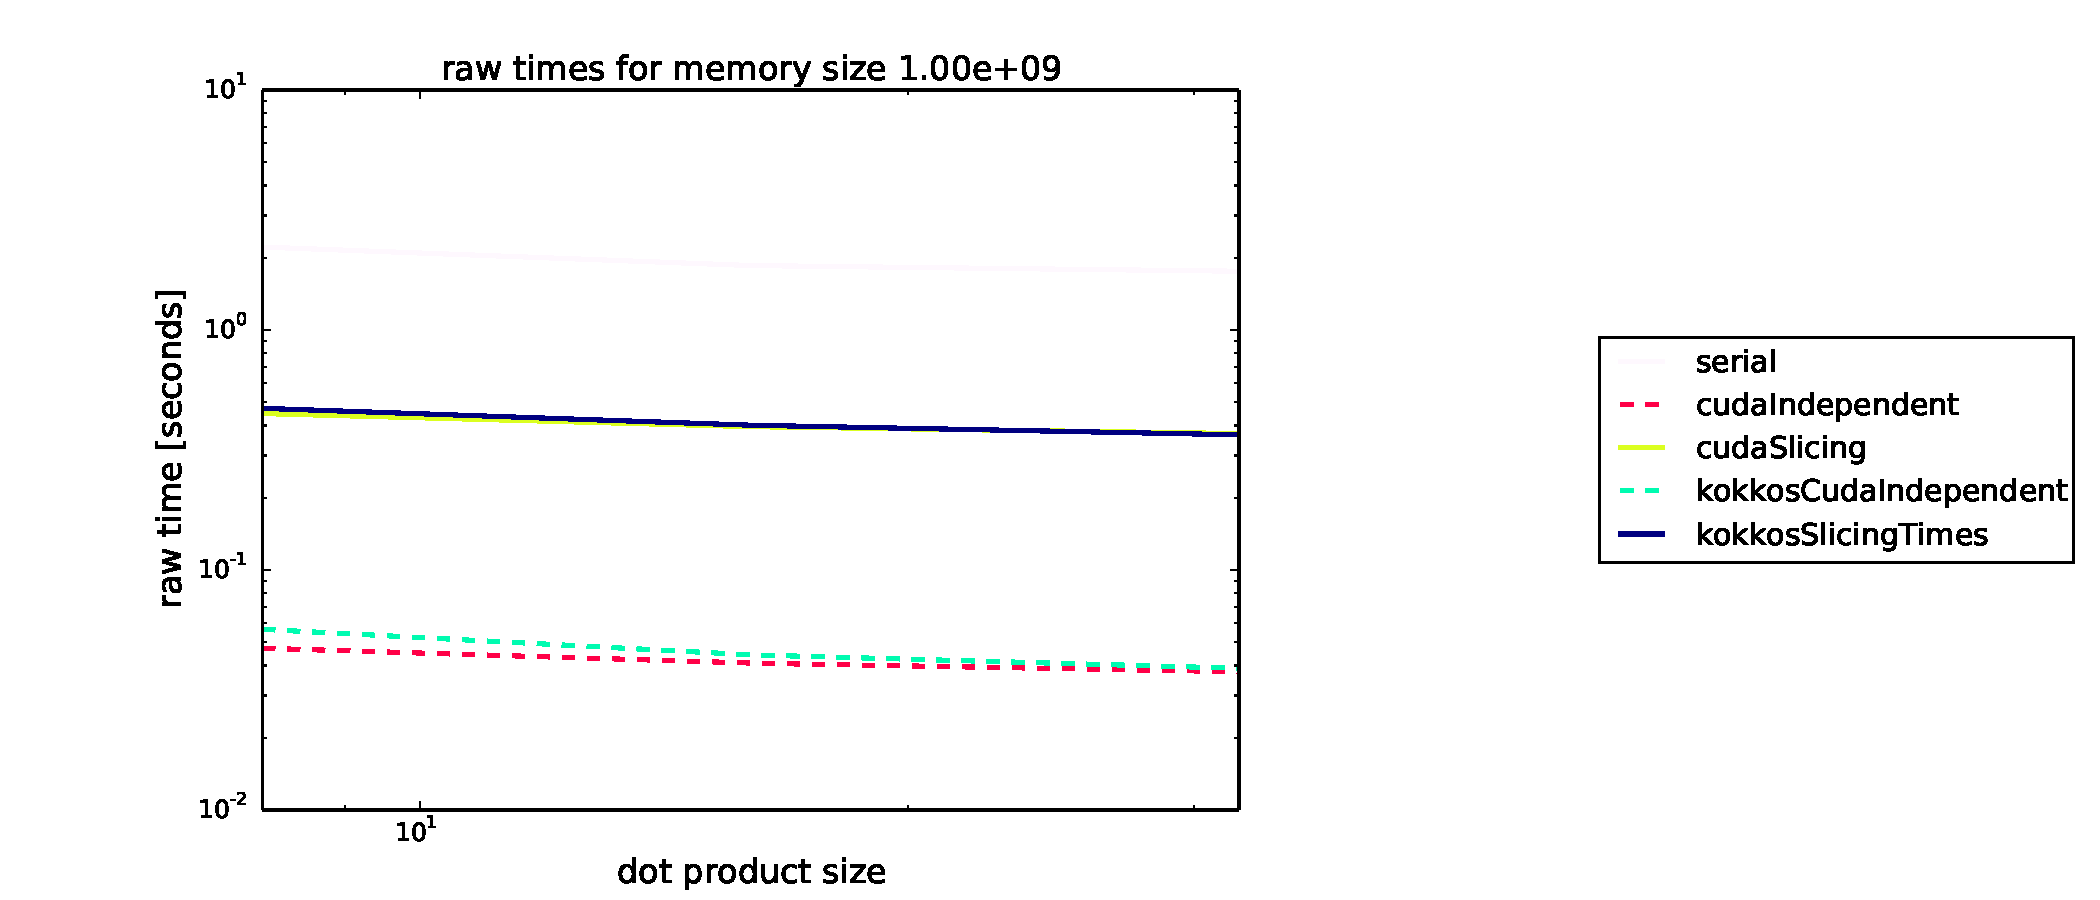
\includegraphics[scale=.4]{CFFS_RawTimes_2d_largest_Comparison.pdf}}
\caption[ContractFieldFieldScalar Kokkos performance comparison]{This graph shows performance differences (or similarities in our case)
of the nested parallelism approach slicing.}
\label{fig:cffscomparison}
\end{figure} \\
In this graph it is clear that the Cuda slicing performance is almost identical
to the Kokkos slicing performance. This is important to show that both Kokkos's
and Cuda's use of shared memory results in the same performance. 

Overall, after seeing a handful of graphs that show Kokkos performs almost
identically to Cuda and to OpenMP, we accepted that Kokkos is not adding any
unneeded overhead. As stated before, there may be slight differences due to
compiler optimizations, but Kokkos seems to perform identically to the other
multithreading solutions.

\section{Snippets}
%Amount of work the programmer has to do is important
%control and complexity of code is important
%Much more complex than OpenMP, but follows a different paradigm
%Very similar to Cuda, except kernel is a functor
%Overall a pretty easy language, some magic values but pretty good
Another major factor that plays into whether or not a programmer uses a certain
language, feature, library, etcetera, is code complexity and ease of coding.
Although this can be subjective, there are a couple differences between the
language we would like to point out, especially regarding amount of code
required compared to Cuda or OpenMP (although comparing to OpenMP may be unfair)
and intuitiveness of the code (or readability). 

Regarding the amount of code required, comparing Kokkos to OpenMP does not seem
fair. Comparing OpenMP to almost anything seems unfair, because OpenMP requires
very little code and most of the work is done for you. Although OpenMP only
works on the CPU which is why it does not require the extra code that Kokkos
requires. In general, OpenMP cannot be compared to Kokkos. If the programmer
knows the code only needs to be multithreaded on the CPU and will never need
more threads then we would strongly advise them to use OpenMP because it is very
simple. However, that is not the niche that Kokkos is trying to fill. 

Kokkos compared to Cuda however, requires similar amounts of code. 
Throughout the code comparison of Cuda and Kokkos we will show
code snippets and point out the differences and similarities directly. We will
start by showing the data setup, because the data needs to get onto the GPU
somehow, then we will move to compare and contrast the Cuda kernel and the Kokkos
functor. \\
\\
Here is code that shows the setup of the data on the GPU for Cuda: \\
\begin{figure}[!htb]
	\begin{lstlisting}
float * dev_leftDataArray;
checkCudaError(cudaMalloc((void **) &dev_leftDataArray, 
	numContractions * numLeftFields * numPoints * 
	sizeof(float)));
	
checkCudaError(cudaMemcpy(dev_leftDataArray, &leftDataArray[0], 
	numContractions * numLeftFields * numPoints * sizeof(float), 
	cudaMemcpyHostToDevice));
	\end{lstlisting}
\caption{Code from Cuda \texttt{ContractFieldFieldScalar}
\label{lst:ContractFieldFieldScalar Cuda Data Setup}}
\end{figure}
\\
There are essentially three steps in the process: declaring a pointer to the
data on the CPU, creating an array with the correct size on the GPU, then
copying the data over to the GPU from wherever the data is currently kept on the
CPU. This process is pretty simple and self-explanatory. Now let us compare that
to Kokkos: \\
\begin{figure}[!htb]
	\begin{lstlisting}
typedef Kokkos::Cuda	DeviceType;
typedef Kokkos::View<float***, Kokkos::LayoutRight, DeviceType>
	ContractionData;
typedef typename ContractionData::HostMirror
	ContractionData_Host;

ContractionData dev_ContractData_Left("left_data",
	numContractions,
	numLeftFields,
	numPoints);

ContractionData_Host contractionData_Left = 
	Kokkos::create_mirror_view(dev_ContractData_Left);

for (int cell = 0; cell < numContractions; ++cell) {
	for (int lbf = 0; lbf < numLeftFields; ++lbf) {
		for (int qp = 0; qp < numLeftFields; ++qp) {
			contractionData_Left(cell, lbf, qp) = 
				contractionDataLeft[cell*numLeftFields*
				numPoints + lbf*numLeftFields + qp];
		}
	}
}
	\end{lstlisting}
\caption{Code from Kokkos Cuda \texttt{ContractFieldFieldScalar}
\label{lst:ContractFieldFieldScalar Kokkos Cuda Data Setup}}
\end{figure}
\\
The Kokkos code first defines and creates the device and host Views. One of the
major differences compared to Cuda is that Kokkos uses its own data structure,
a View, instead of an array. This is why we need to use typedefs to define the
Views, but the extra work (which honestly is not much of a hassle) allows the
programmer much more control over the data. The control also comes at the cost
of having to use for loops to copy the data into the host view instead of being
able to do a Memcpy. However, this is all initial work that needs to be done
once, while the benefit of being able to change the layout of the data by
changing the Kokkos::LayoutRight to Kokkos::LayoutLeft is very useful,
especially since this allows the programmer to optimize data layout for both
the CPU and GPU. Overall, Kokkos' and Cuda's data setup have different
philosophies, which makes sense because Kokkos needs to be easily optimized for
both the CPU and GPU while Cuda only runs on the GPU. 

Looking at the "guts" of the programs, Cuda has a kernel that is launched where
all the computation is, while Kokkos uses a functor, almost identical to
Intel's Thread Building Blocks threading paradigm. However, for programs doing
the same calculation, the parenthesis operator function in Kokkos' functor is
almost an exact replica of the code in Cuda's kernel. Look at the code for a Cuda kernel
for ContractFieldFieldScalar in Figure~\ref{lst:ContractFieldFieldScalar Cuda kernel}: \\
\begin{figure}[htb]
	\begin{lstlisting}
__global__ void
cudaContractFieldFieldScalar_Flat_kernel(int numContractions,
	int numLeftFields,
	int numRightFields,
	int numPoints,
	float * __restrict__ dev_contractData_Left,
	float * __restrict__ dev_contractData_Right,
	float * dev_contractResults) {
	int contractionIndex = blockId.x * blockDim.x + threadIdx.x;
	while (contractionIndex < numContractions) {
		int myID = contractionIndex;
		int myCell = myID / (numLeftFields * numRightFields);
		int matrixIndex = myID % (numLeftFields * 
			numRightFields);
		int matrixRow = matrixIndex / numRightFields;
		int matrixCol = matrixIndex % numRightFields;
		
		// Calculate now to save computation later
		int lCell = myMatrix * numLeftFields * numPoints;
		int rCell = myMatrix * numRightFields * numPoints;
		int resultCell = myMatrix * numLeftFields * 
			numRightFields;
		
		float temp = 0;
		for (int qp =0; qp < contractionSize; qp++) {
			temp += dev_contractData_Left[lCell + 
				qp*numLeftFields + matrixRow] *
				dev_contractData_Right[rCell + 
				qp*numRightFields + matrixCol];
		}

		dev_contractResults[resultCell + 
			matrixRow * numRightFields + matrixCol] = 
				temp;
		
		contractionIndex += blockDim.x * gridDim.x;
	}
}
	
	\end{lstlisting}
\caption{Code from Cuda \texttt{ContractFieldFieldScalar}
\label{lst:ContractFieldFieldScalar Cuda kernel}}
\end{figure} \\
\\
Now compare this to the parenthesis operator code for the Kokkos functor in
Figure~\ref{lst:ContractFieldFieldScalar Kokkos Cuda functor}: \\
\begin{figure}[htb]
	\begin{lstlisting}
KOKKOS_INLINE_FUNCTION
void operator() (const unsigned int elementIndex) const {
	int myID = elementIndex;
	int myCell = myID / (_numLeftFields * _numRightFields);
	int matrixIndex = myID % (_numLeftFields * _numRightFields);
	int matrixRow = matrixIndex / _numRightFields;
	int matrixCol = matrixIndex % _numRightFields;

	float temp = 0;
	for (int qp = 0; qp < _numPoints; qp++) {
		temp += _leftFields(myCell, qp, matrixRow) *
			_rightFields(myCell, qp, matrixCol);
	}
	_outputFields(myCell, matrixRow, matrixCol) = temp;
}
	\end{lstlisting}
\caption{Code from Kokkos Cuda \texttt{ContractFieldFieldScalar}
\label{lst:ContractFieldFieldScalar Kokkos Cuda functor}}
\end{figure}
\\
Although there is some more code for the Kokkos functor (the code required to
declare the data members and the constructor), the Kokkos code looks a lot less
cluttered. The Kokkos functor does not need to deal with figuring out the
thread's ID, because it is an integer given as input, while the Cuda kernel
needs to use blockId.x, blockDim.x, etc. Also indexing into the view is easier,
especially when changing the layout of the data from LayoutLeft to LayoutRight
(or vice versa) because no code changes need to occur in the functor.


\section{Personal Experience and Thoughts}
% Positive experience
% We don't know how to install kokkos and took a while to get things to compile
% Magic word hassles 
% Following examples we can figure out what to do by copying syntax
% No documentation when we wanted to figure out what exactly was happening
% 
A task of the project was to document our experiences and thoughts about Kokkos, including any issues that we have run into. Using new tools and learning new syntax always has its tough periods, and getting used to Kokkos definitely had some periods where we had no idea why a program was not compile or giving an incorrect answer (especially in the beginning), but after the initial learning curve everything seemed to flow pretty well and make sense. 

Our team has never actually been responsible for installing Kokkos on our machine, instead our liaison, Dr. Carter Edwards, did that for us, so we are unable to talk about the difficulties of downloading and installing the Kokkos library on our machine, but we did have lots of trouble trying to compile and linking against Kokkos originally. This was due to the fact that the same flags need to be used when installing and compiling and linking against Kokkos. However, since we did not install Kokkos ourselves and the documentation showing how to compile and link against Kokkos used different flags than what were used during our installation, we struggled for a while. Already this shows how Kokkos' documentation is not as developed as one would like, which we will bring up later, but it is understandable since Kokkos is new. 

Another obstacle that slowed us down when first using, is Kokkos' use of magic
words. For example, Kokkos requires the programmer to typedef Kokkos::Cuda or
Kokkos::OpenMP to device\_type, and it must be device\_type, not some other
name. Although the programmer can easily fix this, if the programmer is unaware
of this requirement it can cause a lot of hassle for a while. Every team member
ran into this at one time or another, but after a while we got used to it. When
following examples we learned to use the same names for the typedefs to make
sure that we did not run into another bug with the same nature. Once again
documentation would have helped in this situation, but there is not much
documentation all we have are examples. On the bright side however, since we
were able to write all of our programs by simply following a few examples we
were able to see some of Kokkos' intuitiveness. Overall we really enjoy Kokkos'
philosophy and structure, which as mentioned before, is almost identical to
Intel's Thread Building Blocks (TBB). If you are familiar with TBB then
learning Kokkos is almost as simple as learning the syntax because they are in
the same paradigm. 

As previously mentioned, Kokkos has very little documentation. For any emerging
technology it is understandable that the creators choose to focus on
functionality instead of documentation, but the documentation needs to catch up
at some point. The examples were very helpful in getting us to our end goal of
working code, but examples are not as helpful in understanding what exactly is
happening, the meaning behind some portions of code, or why certain code is
necessary. Documentation would have also been helpful in seeing the default
values for functions and Views, as well as the other arguments that could have
been passed instead. There were many times we tried to use Google to find
information about Kokkos, but many times the information would point to
uncommented pieces of code, which is not always helpful in determining what is
going on. Overall we believe the documentation for Kokkos needs to improve in
order for new users to get past the initial learning curve and spread the word
about Kokkos. 

As a whole, our team's experience with Kokkos has been positive and see that it
offers a great alternative to other solutions that allow multithreading on
multiple architectures. A quick overview of the benefits of using Kokkos:
Kokkos can create multithreaded code on the CPU, GPU, and XeonPhi, Views can
easily change the layout of the data, functors seem to keep the code cleaner
and more readable than Cuda's kernels, and the fact that Kokkos is a C++
library and not a a new language adds simplicity. Some of the downsides and
changes that we believe would improve Kokkos include Views having more layouts
than LayoutRight and LayoutLeft, the use of magic words (or lack of using the
right magic words) can create bugs that are hard to find, the example code
should include comments to describe what is happening, and finally the
documentation needs to improve. However, extended use of Kokkos will solve most
of these problems except for Views being limited to two layout types, which is
why our team had an overall good experience with Kokkos.

%\begin{table}[ht]
%      \begin{tabular} {| l | l | l | l |l |}
%            \hline
%            & \textbf{Scalar} & \textbf{Vector} & \textbf{Matrix} \\
%            \hline
%			\textbf{1} & $A_{i}\text{ } x \text{ }B_{i} = C$ & $A_{\text{i, j}} \text{ }x \text{ }B_{j} = C_i$  & $A_{\text{i, %j}} \text{ }x \text{ }B_{\text{j, k}} = C_{\text{i, k}}$ \\
%			\hline
%			\textbf{2} & $A_{\text{i, j}} \text{ }x\text{ } B_{\text{i, j}} = C$ & $A_{\text{i, j, k}}\text{ } x\text{ } B_{\text{j, %k}} = C_i$ & $A_{\text{i, j, k}} \text{ }x\text{ } B_{\text{h, j, k}} = C_{\text{i, h}}$ \\
%			\hline
%			\textbf{3} & $A_{\text{i, j, k}} \text{ }x\text{ } B_{\text{i, j, k}} = C$ & $A_{\text{i, j, k, l}}\text{ } x\text{ } %B_{\text{j, k, l}} = C_i$ & $A_{\text{i, j, k, l}} \text{ }x\text{ } B_{\text{h, j, k, l}} = C_{\text{i, h}}$ \\
%            \hline
%        \end{tabular}
%\caption{Summary of the nine Intrepid tensor contraction kernels
%\label{tab:stuff}}
%\end{table}




    % brett
    % Performance 
    % Code snippet

% Tyler

% Expected vs. Actual Performance of this clinic project
\chapter{Our Performance}

The original goal of this clinic project was to parallelize a number of tensor
manipulation kernels in the Intrepid library, and then move on to other kernels
in a different Trilinos library.  However, we have instead focused only on the
tensor manipulation kernels, without having moved on to any other kernels. The
reason for this is twofold:

Firstly, we underestimated the number of obstacles we would encounter over the
course of our project.  Before this project, no member of our team had written
performance-oriented parallel code, forcing us to spend much of the first
semester learning the concepts, techniques, and languages of the field.
However, even as we grew more familiar with parallelizing high-performance code,
we also ran into a number of issues with Kokkos.  Because Kokkos is still a
young project, at the beginning of the semester it had very little
documentation, as well as a few other issues that gave us difficulties.  Over
winter break, we received a newly updated version of Kokkos that included fixes
for some of these issues, along with some new features.

The second reason we did not move on to another package was the Kokkos update we
received over winter break.  The update introduced new functionality, allowing
us to write team-oriented parallel code and implement algorithms such as team
reductions.  The new Kokkos package also gave us access to shared memory on the
GPU. At this point, rather than merely writing flat parallel versions of other
kernels, we decided to focus more heavily on general parallelization techniques
using Kokkos teams for tensor contractions, taking the new Kokkos features into
account.  Thus, because we chose to focus on team techniques, we spent the
spring semester implementing, testing, and plotting results from from various
algorithms as applied to the tensor manipulations library instead of moving to a
different library.

Overall, although our goals diverged from our initial goals as laid out in our 
statement of work, we accomplished a significant amount of exploratory work this
semester. We believe that the work we have acoomplished will be useful to Sandia 
National Laboratories as they continue along the path of making their codebase
thread-scalable.    % tyler


%%% Appendices.

%%% Appendices are just like chapters, only they're generally
%%% lettered rather than numbered (although that depends on your
%%% document class, of course).

%%% The appendices are delineated with the \appendix command.
%%% Individual appendices are begun with the standard \chapter or
%%% \section commands.  In our example, we'll \include them just as
%%% we did other chapters.

%%% If you don't have any appendices, comment out the \appendix
%%% command.

\appendix

\include{our_appendix}

\include{our_source_code}


%%% Back matter.

%%% The back matter of a document is where the bibliography, index,
%%% glossary, and other unnumbered chapters or sections occur.  It
%%% starts, not surprisingly, with the \backmatter command.

\backmatter


%%% Bibliography.

%%% BibTeX is the tool to use for citations and layout of your
%%% bibliography.  Instead of having to type ``[5]'' or ``(Jones,
%%% 1968)'' (and keep track of which citation is which and renumber
%%% them as you add more references to your bibliography), you use
%%% special commands that allow BibTeX and LaTeX to automatically put
%%% the correct information in the right place.

%%% Depending on your field, it may or may not be appropriate to list
%%% references for which you haven't included specific citations.  If
%%% your field sanctions such practices, or if you just want to get an
%%% idea of what you have in your bibliography file, you can include
%%% everything with the \nocite{*} command.
\nocite{*} 


%%% The appearance of your bibliography and citations in your text are
%%% defined by a combination of any bibliography-related LaTeX
%%% packages (such as natbib, harvard, or chicago) and the particular
%%% bibliography style file that you load with the \bibliographystyle
%%% command.  Bibliography-style files end in .bst; you can find them
%%% by searching your file system using whatever tools you have for
%%% doing searches.  (On most modern Unices, ``locate .bst'' will give
%%% you an idea of what's available.)

% Standard bibliography style.
\bibliographystyle{hmcmath}

% Annotated bibliography style.
% \bibliographystyle{hmcmathannote}


%%% The particular bibliography data file or files that you want to
%%% use are specified with the \bibliography file.  Multiple files are
%%% separated by commas.

%%% You might want to use multiple bibliography (or ``bib'') files if
%%% you had a master bib file containing references you use again and
%%% again, and another containing only records for references for a
%%% particular project.

%%% Many people create a single, large bib file that they use for
%%% everything they write.  That approach requires you to \cite every
%%% reference that you want to use in your document -- using
%%% \nocite{*} with a huge bibliography database will give you a large
%%% bibliography containing many references you haven't consulted for
%%% your particular document!

\bibliography{our_bib_file}


%%% Glossary or Index.

%%% If you were going to include a glossary or index in your document,
%%% the relevant commands would appear here.

%%% If you think that you would like to include such features, talk
%%% with someone who's worked with LaTeX a lot very early in your
%%% writing process.  These commands require you to do a bit of
%%% thinking about what you would want to index or gloss in
%%% advance---going back though a completed document to add \index
%%% commands is *not fun*.


\end{document}


